\documentclass[11pt]{article}
\usepackage[a4paper,margin=1in]{geometry}
\usepackage{amsmath,amssymb}
\usepackage{amsthm}
\theoremstyle{definition}
\newtheorem{theorem}{Theorem}
\newtheorem{proposition}{Proposition}
\newtheorem{corollary}{Corollary}
\newtheorem{remark}{Remark}
\newtheorem{example}{Example}
\newtheorem{definition}{Definition}
\usepackage{graphicx}
\usepackage{booktabs,array,calc}
\usepackage[font=small,labelfont=bf]{caption}
\usepackage[colorlinks=true]{hyperref}
\providecommand{\tightlist}{\setlength{\itemsep}{0pt}\setlength{\parskip}{0pt}}
\setcounter{secnumdepth}{-1}
\emergencystretch=3em

\begin{document}

\title{Supplementary Material: Obstruction certificates under incomplete observation}
\author{Amin Abaee\\[0.2em]{\small Independent Researcher}}
\maketitle

This supplement collects the material condensed from the main text: selected Section 3 certificate proofs (S1 and S2), the expanded sufficiency review (S2), the bounded constructions and scope remarks (S3), and three additional figures (S4). S1 collects selected proofs and worked certificates of the main text's statements --- including the selector principle, the sparse common-action witness, and the soundness of the oracle-recourse certificate (stated with its display in the support-function form) --- together with the extended discussions and worked instances of the main text's Sections 3, 4, and 10, as the closing blocks of this section. Notation follows the main article, but theorem, proposition, remark, table and figure numbering is independent in this document. A selected concordance is: article Theorems 1/2/3/5 correspond to supplementary Theorems 1/2/3/4; article Theorem 4 has its indexed LP proof in S2; article Propositions 2/3 correspond to supplementary Propositions 1/2; article Proposition 6 has its recourse proof in S1; article Proposition 9 has its two-phase argument in S2. The main article's Section 3.8 aggregate LP has no matching supplementary theorem. These article-to-supplement locations are source-level only and require checking against compiled paginated proofs. This is an unrefereed author draft; the continuous original-path premises and sensor-specific regularity are not certified by the finite formalization.

\section*{S1. Certificates and detailed proofs}

\begin{theorem}[finite-horizon soundness and completeness]\label{thm:finite-horizon}
An initial post-observation cell \(B_0\) admits an observation-based
policy that keeps every compatible trajectory in \(\mathcal V\) for
\(N\) steps if and only if \(B_0\in\mathcal W_N\). A prior
\(P\) is viable if and only if every nonempty initial observation cell
\(P\cap O^{-1}(y)\) belongs to \(\mathcal W_N\).
\end{theorem}

\emph{Proof.} The initial observation partitions a prior into
disjoint cells; one policy may choose independently on each cell. It
therefore suffices to prove the post-observation statement.
\((\Rightarrow)\) Induction on \(N\). The case \(N=0\) is
\(B_0\subseteq\mathcal V\), i.e.\ \(B_0\in\mathcal W_0\). If a policy is
safe for \(N\) steps, its first action \(a\) is admissible at every
compatible state, so \(a\in U^B(B_0)\); for every possible observation
\(y\), the successor belief \(\mathrm{Post}(B_0,a,y)\) is safe for \(N-1\)
steps under the same policy, so by induction
\(\mathrm{Post}(B_0,a,y)\in\mathcal W_{N-1}\); hence
\(B_0\in\mathrm{Pre}(\mathcal W_{N-1})=\mathcal W_N\).

\((\Leftarrow)\) Backward induction. If \(B_k\in\mathcal W_{N-k} =
\mathrm{Pre}(\mathcal W_{N-k-1})\), choose the witness action
\(a_k\in U^B(B_k)\); after the observation \(y_k\) the successor belief
\(B_{k+1}=\mathrm{Post}(B_k,a_k,y_k)\in\mathcal W_{N-k-1}\), and the
recursion continues. By construction every reachable state over \(N\)
steps lies in \(\mathcal V\). \ensuremath{\square}

\begin{theorem}[common-action obstruction]\label{thm:common-action}

Let \(B \subseteq \mathcal{V}\) be an information set of the specified observation structure (the safe-control correspondence
\(\mathcal{R}_{\mathcal{V}}\) is defined on \(\mathcal{V}\), so the
belief is taken inside it). Suppose the following hypotheses hold.

(H2.1) The selected action is held until the next observation (sampled
review: no informative observation arrives before the next action must
be selected, and the policy holds the selected action over the review
interval --- the institutional reading; without a positive dwell time
the instantaneous statement below must be replaced by the tube-safety statement below).

(H2.2) Either the \textbf{common admissible action set} is empty,
\[U^B(B) \;=\; \bigcap_{x \in B} U(x) \;=\; \varnothing, \qquad \text{(admissibility obstruction)}\]
or the \textbf{common safe-action set} is empty while common
admissibility holds,
\[\mathcal{R}_{\mathcal{V}}^B(B) \;:=\; \bigcap_{x \in B} \mathcal{R}_{\mathcal{V}}(x) \;=\; \varnothing \quad \text{with} \quad U^B(B) \neq \varnothing, \tag{1} \qquad \text{(safety obstruction)}\]

(H2.3) \textbf{Compatible original-system adverse path.} In the safety case, for every candidate held \(a\in U^B(B)\) there exist a compatible boundary state \(x_a\), an active constraint \(j_a\), constants \(c_a,\tau_a>0\), and an admissible original-system Carath\'eodory pair under \(a\), with \(d_a(t)\in D(x_a(t))\) and \(q_{j_a}(x_a(t))\le-c_a t<0\) for \(0<t<\tau_a\) before any informative observation. This premise is about a realized path and does not follow merely from the closed graph or ambient lower semicontinuity of \(D\); a convexified-inclusion trajectory is not substituted for an original path.

Then, under hypotheses (H2.1)--(H2.3),
\(B \notin \mathrm{ERViab}_{\mathcal{I}}(\mathcal{V})\): every
compatible state may be individually robustly viable, and the belief is
nevertheless nonviable, because the state-specific safe actions are
incompatible.

\end{theorem}

\emph{Proof.} Let \(\pi\) be any observation-based policy, and let
\(a = \pi(B)\) be the action it selects at the information set \(B\).

\textbf{Admissibility case.} If \(a \notin U^B(B)\), then for some
compatible state \(x \in B\) the action is inadmissible
(\(a \notin U(x)\)): at that state the selected action is not an
admissible control, so the policy fails outright on the compatible
branch from \(x\) --- an obstruction independent of the safe set.

\textbf{Safety case.} Otherwise \(a\in U^B(B)\). Since the active-gradient response equals \(U(x)\) at interior points, its empty common intersection implies that this particular command fails an active boundary inequality at a compatible state. Hypothesis (H2.3) provides a \emph{realized original-system} path from such a state whose corresponding active constraint becomes strictly negative at arbitrarily small positive times, before the next review. Thus this policy fails on one admissible compatible path. The policy was arbitrary within the required hold class; no claim is made for within-review switching or for relaxed-only paths. \ensuremath{\square}

\begin{proposition}[uniform margin gives a tube obstruction at every review length]\label{prop:uniform-margin}
Let \(B\subseteq\mathcal V\) be a compact information set with
\(U^B(B)\neq\varnothing\), \(f\) and \(\nabla q_j\) continuous, and
suppose there is \(\eta>0\) such that for every \(a\in U^B(B)\) there
exist a boundary state \(x_a\in B\cap\partial\mathcal V\), an active
constraint \(j\) with \(q_j(x_a)=0\), and a disturbance \(d_a\in D(x_a)\)
satisfying
\[\nabla q_j(x_a)\cdot f(x_a,a,d_a) \le -\eta.\]
Assume for each candidate command the original-system adverse path (H2.3) at the relevant state. Then the tube-safe action set is empty
at every review length,
\[\mathcal{A}_{\mathrm{tube}}(B,\Delta)=\varnothing \qquad \forall\,\Delta>0,\]
and hence \(B\notin\mathrm{ERViab}_{\mathcal I}(\mathcal V)\) under
sampled review of any length.
\end{proposition}

\emph{Proof.} Fix a candidate held command \(a\). By the assumed compatible original-system path, its active floor becomes negative on some interval \((0,\tau_a)\). Every \(\Delta>0\) contains a time in that interval, so \(a\notin\mathcal A_{\mathrm{tube}}(B,\Delta)\); no lower bound on \(\tau_a\) uniform in \(a\) is needed. Exhausting the common candidate set proves the assertion only for the class obliged to hold for that review. \ensuremath{\square}

\begin{proposition}[obstruction ladder]\label{prop:ladder}
For the declared held-action review class, with original-system exiting paths (H2.3) whenever an active-gradient test fails, the common response sets
of Section 2.4 are nested:
\[\mathcal{A}_{\mathrm{tube}}(B,\Delta) \;\subseteq\; \mathcal{R}_{\mathcal{V}}^B(B) \;\subseteq\; U^B(B) \qquad \forall\,\Delta>0,\]
and emptiness descends the ladder:
\[U^B(B)=\varnothing \;\Longrightarrow\; \mathcal{R}_{\mathcal{V}}^B(B)=\varnothing \;\Longrightarrow\; \mathcal{A}_{\mathrm{tube}}(B,\Delta)=\varnothing \;\Longrightarrow\; B\notin\mathrm{ERViab}_{\mathcal{I}}(\mathcal{V}).\]
\end{proposition}

\emph{Proof.} The second inclusion follows from \(\mathcal R_{\mathcal V}(x)\subseteq U(x)\). For the first, if \(a\in U^B(B)\) fails an active-gradient inequality at a compatible boundary state, (H2.3) gives an admissible original-system path with \(q_j(x(t))<0\) arbitrarily soon; hence it cannot be tube-safe. A constant \(d\in D(x_0)\) need not remain admissible as \(x(t)\) moves when \(D\) depends on state. Emptiness of the held-command tube rules out a policy \emph{required} to hold that same command for this review; it does not rule out a time-varying input signal. The discrete \(\mathcal A_N\) is not included in the continuous tube without a defined sampled-transition bridge. \ensuremath{\square}

\begin{theorem}[delayed-information obstruction]\label{thm:delayed}

Let \(B_0\) be an initial post-observation information cell whose
members share a current reading. Suppose the following
hypotheses hold.

(H3.1) Fix a blind interval \([0,T_{\mathrm{obs}})\) with
\(T_{\mathrm{obs}}>0\). For each implementable control history in the
declared class, \emph{every} compatible realization while safe produces
the same observation record on this interval (up to its first exit).
Thus no branch-dependent observation can change the policy's control
before exit; the set-membership information state may evolve, but the
common record contains no branch-discriminating signal.

(H3.2) Fix the class being certified: by default all implementable measurable blind-window controls; a declared whole-window hold class yields only class-relative nonviability. There is a function \(q\) of class \(C^1\), defined on a neighbourhood of
the relevant trajectories, with \(\mathcal V\subseteq\{q\ge0\}\),
and \(\varepsilon>0\). Let \(B_0\subseteq\mathcal V\) be compact,
and fix \(a>\max_{B_0}q\ge0\).
\textbf{For every implementable blind-window control} \(u(\cdot)\) in the
declared class, measurable and common to all compatible states while
there is no informative observation, there exist a minimizer
\(x_u\in B_0\) of \(q\) and an admissible disturbance realization
with an absolutely continuous solution from \(x_u\). This solution
exists through any first contact with \(q=0\) until either it reaches
\(q<0\) or \(T_{\mathrm{obs}}\), and follows the common record
of (H3.1) until exit. For almost every pre-exit time in the closed strip
\(0\le q(x(t))\le a\), \emph{including boundary contact},
its actual derivative obeys
\[\frac{d}{dt}q(x(t))=\nabla q(x(t))\cdot f(x(t),u(t),d(t))
\;\le\;-\varepsilon. \tag{2}\]
The realization is chosen \emph{after} \(u\), not before it. This
condition is on a genuine admissible trajectory of the original system,
not solely on a convexified disturbance inclusion; no exit is assumed
in the hypothesis. It may fail even when a positive-side drift estimate
holds.

(H3.3) The timing bound holds:
\[T_{\mathrm{obs}} \;>\; \frac{\inf_{x \in B_0} q(x)}{\varepsilon}. \tag{3}\]

Then under (H3.1)--(H3.3), no policy in the fixed class is viable
from \(B_0\). For the unrestricted observation-based class this yields
\(B_0\notin\mathrm{ERViab}_{\mathcal I}(\mathcal V)\); for a proper
institutional subclass it does not exclude unrestricted viability.

\end{theorem}

\emph{Proof.} Fix a policy in the declared class. Hypothesis (H3.1)
gives it a common blind control \(u\); an action inadmissible on a
compatible branch already fails. Otherwise (H3.2) supplies a compatible
minimizer and a genuine adverse trajectory. Put
\(h(t)=q(x(t))\), \(h(0)=m=\min_{B_0}q\ge0\), and
\(t_*=m/\varepsilon<T_{\mathrm{obs}}\). Suppose there is no strict
violation by some \(t_1\in(t_*,T_{\mathrm{obs}})\). As long as
\(0\le h\le a\), (2) gives \(h(t)\le m-\varepsilon t\).
The trajectory cannot first leave this strip through \(h=a\) because
its derivative is strictly negative there almost everywhere; at a
contact \(h=0\) it cannot remain nonnegative through \(t_1\)
for the same reason. Hence nonviolation through \(t_1\) would give
\(0\le h(t_1)\le m-\varepsilon t_1<0\), a contradiction.
This includes \(m=0\): contact alone would not violate the closed constraint; negative drift while still safe is required at the boundary,
not a vacuous condition on \(h>0\). The realization continues through
first contact by (H3.2), so some \(t<t_1<T_{\mathrm{obs}}\) has
\(q(x(t))<0\), contrary to safety. The policy was arbitrary; the
quantifier is \(\forall\pi\,\exists(x_u,d_u)\), not a demand that
every trajectory drift downward.
Only an unrestricted blind-control class licenses the conclusion for the
full observation-based kernel; a declared hold class does not.

\begin{theorem}[finite-time exit certificate]\label{thm:exit}

Let \(q : X \to \mathbb{R}\) be a constraint function of class \(C^1\) --- the class assumed throughout the exit theorems --- with
\(\mathcal{V} \subseteq \{ q \ge 0 \}\), and suppose the following
hypotheses hold.

(H5.1) There exist constants \(a > 0\) and \(\varepsilon > 0\) such that
on the strip \(\mathcal{S}_a = \{ x : 0 \le q(x) \le a \}\),
\[\sup_{u \in U(x)} \inf_{d \in D(x)} D^+ q(x; f(x,u,d)) \;\le\; -\varepsilon \qquad \forall x \in \mathcal{S}_a, \tag{4}\]
where \(D^+ q(x; v) = \limsup_{h \downarrow 0} [q(x + hv) - q(x)]/h\) is
the upper right Dini derivative of \(q\) in direction \(v\) (for \(C^1\)
\(q\), \(D^+ q(x; v) = \nabla q(x) \cdot v\) --- the form the proof
uses).

(H5.2) \textbf{Compatible original-system adverse pair.} For each admissible control history in the declared class and each initial state in \(\mathcal S_a\), assume an absolutely continuous original-system state and measurable disturbance exist, with \(d(t)\in D(x(t))\), \(\dot x=f(x,u(t),d(t))\) almost everywhere, and \(\dot q(x(t))\le-\varepsilon\) almost everywhere while \(0\le q(x(t))\le a\) before exit. This pair continues through first boundary contact until strict exit or beyond \(q(x_0)/\varepsilon\). Ambient lower semicontinuity and closed graph alone are not claimed to supply this path; a convexified path alone does not witness the original game.

Then the infimum of strict-violation times along such a path is at most \(q(x_0)/\varepsilon\). For every later deadline a strict violation occurs before that deadline, so the declared control class is nonviable from \(\mathcal S_a\); strict exit \emph{at} the bound is not asserted. Theorem 4 is independent of an observation argument but conditional on (H5.2) and its chosen policy class.
\end{theorem}

\emph{Proof.} Fix the control and original pair. If it stayed in \(q\ge0\) through any \(t_1>q(x_0)/\varepsilon\) before the assured continuation ends, it could not exit the strip upward through \(q=a\). Integrating only on the safe part of the closed strip gives \(0\le q(x(t_1))\le q(x_0)-\varepsilon t_1<0\), a contradiction. Thus a strict violation occurs before every later deadline. No use is made of a thresholded-correspondence LSC inheritance or an unproved closed-loop selection. \ensuremath{\square}

\begin{proposition}[epistemic emptiness by admissibility --- a minimal construction]\label{prop:emptiness}

There exists a system with
\(\mathrm{Viab}(\mathcal{V}; U, \pi_{\mathrm{perf}}) = \mathcal{V} \neq \varnothing\)
such that, for a non-injective observation map \(O\), every \emph{full-fibre} initial information state --- the observation fibres
\(B_0 = O^{-1}(O(S_0))\), \(S_0 \in \mathcal{V}\) --- lies outside
\(\mathrm{ERViab}_{\mathcal{I}}(\mathcal{V})\): the epistemic kernel
over the fibre-induced initial beliefs is empty. The mechanism is a state-dependent-admissibility-induced \emph{safety obstruction}, not an empty common admissible set: the
state-dependent control set of the construction leaves a single common
action at the merged belief --- one that is outward-drifting at the
boundary state --- so the emptiness is the common-action obstruction
(Theorem~\ref{thm:common-action}'s safety case) at minimal size, produced by the control-set primitive rather than by information; the
hidden-mode instance is Example~\ref{ex:hidden-mode}.

\end{proposition}

\emph{Proof (by construction).} Let \(X = [1,2]\), \(\dot S = u - r(S)\)
with \(r : [1,2] \to \mathbb{R}_{++}\) continuous and \textbf{injective
on \([1,2]\)} (e.g.~\(r(S) = S - 1 + c\), \(c > 0\), strictly
increasing), the unrelaxed nonconvex \(U(S) = \{0, r(S)\}\), \(\mathcal{V} = [1,2]\), and the
constant observation \(O(S) \equiv 0\). Under perfect information, the
state-feedback control \(u = r(S)\) gives \(\dot S = 0\), so every
\(S_0 \in \mathcal{V}\) is viable:
\(\mathrm{Viab}(\mathcal{V}; U, \pi_{\mathrm{perf}}) = \mathcal{V}\).
Under the constant observation, the initial information state is the
fibre \(B_0 = [1,2]\), and the set-membership semantics propagates it:
at time \(t\) the belief is \(B_t = \Phi_t(B_0) \cap \mathcal{V}\), the
image of the initial set under the flow generated by the applied control
--- under a constant observation with no exit observation, this
flow-image coincides with the record-compatibility definition of Section
2.3. The common control set at the initial belief is
\[U^B(B_0) = \bigcap_{S \in [1,2]} \{0, r(S)\} = \{0\},\] because
\(r(S) > 0\) for every \(S\) and, by injectivity on \([1,2]\), no single
control equals \(r(S)\) for all \(S\). An observation-based policy may
select time-varying actions, but robust admissibility requires the
selected action to lie in \(U^B(B_t)\) at every \(t\); the propagated
belief \(B_t\) is nonempty and, while the state remains in \([1,2]\),
\(U^B(B_t) = \{0\}\) by the same computation (the flow of
\(\dot S = -r(S)\) with \(r > 0\) moves \(B_t\) monotonically downward,
preserving the injectivity of \(r\) on the surviving interval). Hence
the policy must hold \(u(t) = 0\) almost everywhere, giving
\(\dot S = -r(S) \le -\min_{[1,2]} r < 0\); every compatible trajectory
exits \(\mathcal{V}\) downward in finite time. The same argument applies
verbatim to any initial fibre, since \(O\) is constant. Hence
\(\mathrm{ERViab}_{\mathcal{I}}(\mathcal{V})\) contains no fibre-induced
initial belief, while a singleton prior under the same constant sensor can be viable and must not be excluded from the common ambient belief domain. The empty-kernel statement is restricted to full-fibre starting beliefs. The system has no disturbance and no estimation error: the
failure is caused entirely by the non-injectivity of \(O\). \ensuremath{\square}

\begin{proposition}[observation-fibre criterion]\label{prop:fibre}

An exact certifier
based on \(O\) exists if and only if membership in \(K\) is constant on
every observation fibre:
\[O(z_1) = O(z_2) \;\Longrightarrow\; \big[ z_1 \in K \iff z_2 \in K \big] \qquad \forall z_1, z_2 \in Z, \tag{5}\]
equivalently, \(K = O^{-1}(O(K))\) on the admissible domain.

\end{proposition}

\emph{Proof.} (\(\Rightarrow\)) If \(C\) exists and \(O(z_1) = O(z_2)\),
then \(\mathbf{1}_K(z_1) = C(O(z_1)) = C(O(z_2)) = \mathbf{1}_K(z_2)\),
so membership is fibre-constant.

(\(\Leftarrow\)) If (5) holds, define \(C(y) = \mathbf{1}_K(z)\) for any
\(z \in Z\) with \(O(z) = y\); (5) makes \(C\) well defined on \(O(Z)\)
and exact by construction; extend \(C\) arbitrarily on
\(Y \setminus O(Z)\). A \emph{measurable} exact certifier exists under
the same condition on standard Borel spaces when \(O(K)\) is measurable,
taking \(C = \mathbf{1}_{O(K)}\); measurability is the only additional requirement. \ensuremath{\square}

\begin{corollary}[safety-crossing fibres and the certainly-safe set]\label{cor:certainly-safe} If two admissible states share an observation and lie on opposite
sides of the \emph{same} component safety constraint --- with the safe
set of that certification problem read as the single floor
\(K = \{ q_j \ge 0 \}\); or, in the general form of the hypothesis, one
of the two states lies in \(K\) and the other outside \(K\) --- no exact
observation-only certificate exists. (Crossing one floor of an
intersection \(K = \bigcap_j \{ q_j \ge 0 \}\) does not by itself put
the pair on opposite sides of the intersection --- the state satisfying
floor \(j\) may violate floor \(i\) --- hence the single-floor scoping.)
The largest set of observations that can soundly be labeled safe without
further information is the certainly-safe set
\[\mathcal{Y}_{\mathrm{safe}} \;=\; \big\{ y \in O(Z) : O^{-1}(y) \subseteq K \big\}.\]

\end{corollary}

\emph{Proof.} In the general form (one state in \(K\), one outside), the
fibre violates (5) for that \(K\), so Proposition~\ref{prop:fibre} denies the certifier; in
the single-floor form it violates (5) for the floor's own certification
problem (\(K = \{q_j \ge 0\}\)). On \(\mathcal{Y}_{\mathrm{safe}}\)
every compatible state is safe, so the constant verdict ``safe'' is
sound; outside \(\mathcal{Y}_{\mathrm{safe}}\) some compatible state is
unsafe, so no sound ``safe'' verdict exists there. \ensuremath{\square}

\begin{proposition}[monotonicity of the epistemic kernel]\label{prop:monotone}
The robust epistemic kernel is monotone in its constituents: enlarging
the action sets, reducing the disturbance sets, refining the information
structure, or enlarging the policy class never shrinks the kernel.
Writing \(\mathrm{ERViab}^{\,\cdot}\) for the kernel with the indicated
constituent, \(U_1\subseteq U_2\), \(D_1\subseteq D_2\),
\(\Pi_1\subseteq\Pi_2\), and ``\(\mathcal{I}_1\) refines
\(\mathcal{I}_2\)'' imply respectively
\[\mathrm{ERViab}^{U_1} \subseteq \mathrm{ERViab}^{U_2}, \qquad
\mathrm{ERViab}^{D_2} \subseteq \mathrm{ERViab}^{D_1},\]
\[\mathrm{ERViab}^{\Pi_1} \subseteq \mathrm{ERViab}^{\Pi_2}, \qquad
\mathrm{ERViab}^{\mathcal{I}_2} \subseteq \mathrm{ERViab}^{\mathcal{I}_1}.\]
This refinement inclusion compares kernels on the \emph{same domain of prior beliefs}; it is not a literal inclusion of differently typed already-observed fibres.
\end{proposition}

\emph{Proof.} Each inclusion is by restriction: a policy that is viable
under the smaller action sets, the larger disturbance sets, the smaller
policy class, or the coarser information structure remains admissible
and nonanticipative under the corresponding enlargement or refinement,
while the adversary's options are unchanged or reduced, so the same
policy witnesses viability. \ensuremath{\square}

\noindent\textbf{Complete proof of the selector principle (main text, Section 8).}
Let \(\pi\) witness \(B \in \mathrm{ERViab}_{\mathcal{I}}(\mathcal{V})\).
(i) \emph{Admissibility.} The policy \(\pi\) is admissible by the
definition of epistemic viability, so its review selection
\(a = \pi(B)\) satisfies \(a \in U(x)\) for every compatible
\(x \in B\) --- an admissible policy never selects an action outside the
state-dependent control set at a reachable state --- whence
\(a \in U^{B}(B)\). (ii) \emph{Safety.} Every trajectory compatible with
\(B\) and governed by \(\pi\) over the review interval \([t_{k},
t_{k} + \Delta]\) lies in \(\mathcal{V}\); under the sampled-hold
semantics the union of these segments over compatible initial states is
exactly \(\mathrm{Reach}_{[0,\Delta]}(B, a)\), giving the inclusion
\(\mathrm{Reach}_{[0,\Delta]}(B, a) \subseteq \mathcal{V}\). (iii)
\emph{Recursive viability.} Let \(B' = \tau(B, a, y)\) be any
post-observation belief reached at the next review. Every \(x \in B'\)
lies on a trajectory compatible with the observation record through
\(t_{k} + \Delta\) that stayed in \(\mathcal{V}\) so far and is governed
beyond \(t_{k} + \Delta\) by the continuation of \(\pi\); that
continuation is admissible, information-adapted, and keeps every such
trajectory in \(\mathcal{V}\) --- otherwise \(\pi\) would fail to keep
every compatible trajectory of \(B\) in \(\mathcal{V}\) on
\([0, \infty)\). Hence \(\pi|_{B'}\) witnesses
\(B' \in \mathrm{ERViab}_{\mathcal{I}}(\mathcal{V})\), which is (iii).
Induction on the review index now shows that all four response
correspondences --- \(U^{B}\), \(\mathcal{R}_{\mathcal{V}}^{B}\),
\(\mathcal{A}_{\mathrm{tube}}\) at the review length, and the recursive
predecessor --- are nonempty at every reachable belief, each containing
\(\pi\)'s review selection; by contraposition, a certificate that any
one of them is empty at a reachable belief certifies nonviability. The
finite-system converse is the backward induction of
Theorem~\ref{thm:finite-horizon} applied to the review-time belief
recursion. The continuous-time converse is the backward-recursion
completion recorded in Section 6.5 of the main text; it is cited there
and not re-derived. \rule{0.5\linewidth}{0.5pt}

\bigskip
\noindent\textbf{Complete proof of the sparse common-action witness
(main text, Section 3; Proposition 4 of the main article).}
This proves the \emph{same tangent-condition statement} as the main
text, not a separate discrete successor condition. At a fixed state
\(x\), let \(J(x)\) denote the active safety facets, and use safety
\(q_j\ge0\) and the control-affine vector field
\(f(x,u,d)=f_0(x,d)+f_u(x,d)u\). Then
\[\mathcal R_{\mathcal V}(x)=\{u\in U(x):
\nabla q_j(x)\cdot f(x,u,d)\ge0\quad
\forall j\in J(x),\ \forall d\in D(x)\}.\]
For each fixed \((x,j,d)\) the expression on the left of the
inequality is affine in \(u\). Thus the inequality defines a closed
halfspace in control space, regardless of whether \(q_j\) is convex
as a function of \(x\). Intersecting these halfspaces over all active
facets and disturbances with the closed convex admissible set \(U(x)\)
gives a closed convex set. Since \(U(x)\subseteq U\) and \(U\) is
compact, the set is compact (including when it is empty). Now suppose
\(\bigcap_{x\in B}\mathcal R_{\mathcal V}(x)=\varnothing\).
Each member of the family \(\{\mathcal{R}_{\mathcal{V}}(x)\}_{x \in B}\)
is compact and convex in the Euclidean space \(U \subseteq
\mathbb{R}^{m}\). If every finite subfamily had nonempty intersection,
the finite-intersection property of the compact sets would give nonempty
total intersection --- contradiction; so some finite subfamily
\(\mathcal{R}_{\mathcal{V}}(x_{1}), \dots,
\mathcal{R}_{\mathcal{V}}(x_{N})\) has empty intersection. By Helly's
theorem in \(\mathbb{R}^{m}\) (Helly, 1923), a finite family of convex
sets in \(\mathbb{R}^{m}\) with empty intersection contains a
subfamily of at most \(m + 1\) members with empty intersection; the
corresponding \(x_{1}, \dots, x_{\ell}\), \(\ell \le m + 1\), are the
required witness. The converse direction is immediate --- the witness
sets are members of the family, so their empty intersection implies the
full one. \smallskip

\emph{Scope of the convexity hypothesis.} For the continuous-time
tangent condition just proved, convexity is required of \(U(x)\)
and of the resulting control sets, \emph{not} of \(q_j(x)\):
\(C^1\) regularity suffices for the affine-in-control tangent
inequalities. A different, discrete rule based on
\(q_j(F(x,u,d))\ge0\) need not produce convex control sets without
additional hypotheses; that rule is not the proposition proved here.
\rule{0.5\linewidth}{0.5pt}

\bigskip
\noindent\textbf{Complete proof of the soundness of the oracle-recourse
certificate (main text, Section 3.7), with the display corrected to the
support-function form.}
Use the main proposition's narrowed hypotheses: for each fixed exogenous
admissible disturbance scenario the state equation is affine in the state
and input with coefficients independent of the controlled path, and each
stored facet \(g_j(x)=c_j^\top x+b_j\) is affine with safety
\(g_j\ge0\). Thus \(\beta_\ell^d=g_j(\bar x_\theta^d(t))\) is its
zero-control facet value. For signals \((w,u_\theta)\) --- \(w\) common
on \([0,\tau)\), \(u_\theta\) a branch's post-reveal signal ---
variation of constants and affinity of \(g_j\) give the following
\emph{exact} identity. General control-affine dynamics with
state-dependent \(B(x)\), or nonlinear facets, are not covered without
a separately validated one-sided remainder bound:
\[
g_{j}\bigl(x_{\theta}^{u, d}(t)\bigr) \;=\; \beta_{\ell}^{d}
\;+\; \int_{0}^{\tau} \bigl(k_{\ell}^{d}\bigr)^{\top} w
\;+\; \int_{\tau}^{t} \bigl(k_{\ell}^{d}\bigr)^{\top} u_{\theta},
\]
the kernel \(k_{\ell}^{d}\) exactly as defined in the main text.
\emph{Corrected certificate.} Define, for weights
\(\lambda_{\ell} \ge 0\), \(\sum_{\ell} \lambda_{\ell} = 1\),
\[
\Gamma_{h}(\lambda) \;=\; \inf_{d(\cdot)} \Bigl\{ \sum_{\ell}
\lambda_{\ell} \beta_{\ell}^{d} \;+\; \int_{0}^{\tau}
h_{U}\Bigl(\sum_{\ell} \lambda_{\ell} k_{\ell}^{d}\Bigr)\, d\sigma
\;+\; \sum_{\ell} \int_{\tau}^{T} h_{U}\bigl(\lambda_{\ell}
k_{\ell}^{d}\bigr)\, d\sigma \Bigr\},
\]
with \(h_{U}(g) := \max_{v \in U} g^{\top} v\) the support function. If
\(\Gamma_{h}(\lambda) < 0\), then \(B_{0} \notin
\mathrm{ERViab}_{\mathcal{I}}(\mathcal{V})\): for every policy,
at least one compatible stored branch has a violated facet under the
fixed exogenous scenario (the branch may depend on the policy).
\emph{Proof.} Since \(\Gamma_h<0\), the definition of infimum supplies
one exogenous admissible scenario \(d^{*}(\cdot)\) whose bracket is
strictly negative. That same scenario is admissible against every
policy; attainment of the infimum is unnecessary. Consider any
admissible policy: its window signal \(w\) is one fixed measurable
function (the blind-window reduction of
Theorem~\ref{thm:delayed}), and its post-reveal branch signals
\(u_{\theta}\) are arbitrary measurable functions. The realized
weighted facet sum at \(d^{*}\) is
\[
\sum_{\ell} \lambda_{\ell} g_{j_{\ell}}\bigl(x_{\theta_{\ell}}(t_{\ell})
\bigr) \;=\; \sum_{\ell} \lambda_{\ell} \beta_{\ell}^{d^{*}}
\;+\; \int_{0}^{\tau} \Bigl(\sum_{\ell} \lambda_{\ell}
k_{\ell}^{d^{*}}\Bigr)^{\top} w \;+\; \sum_{\ell} \int_{\tau}^{t_{\ell}}
\bigl(\lambda_{\ell} k_{\ell}^{d^{*}}\bigr)^{\top} u_{\theta_{\ell}},
\]
and each pairing is bounded above by the support function,
\(g^{\top} v \le h_{U}(g)\) for \(v \in U\). Hence the realized weighted
facet sum is at most
\(\sum_{\ell} \lambda_{\ell} \beta_{\ell}^{d^{*}} + \int_{0}^{\tau}
h_{U}(\sum_{\ell} \lambda_{\ell} k_{\ell}^{d^{*}}) + \sum_{\ell}
\int_{\tau}^{T} h_{U}(\lambda_{\ell} k_{\ell}^{d^{*}}) < 0\). A strictly
negative weighted sum of the facet values forces some facet value to be
strictly negative: the facet is violated along its branch. Since the
window signal \(w\) was arbitrary, every policy in the class fails;
the violating stored branch can depend on the policy; no assertion
about every individual branch is needed. \(\square\)

\emph{Remark (an attainment-special variant).} A variant certificate
replaces \(h_{U}\) by the minimum \(\phi_{U}(g) = \min_{v \in U}
g^{\top} v\) and the firing inequality by the opposite sign. That form
is sound exactly when the realized control pairings attain their
pointwise minima, i.e.\ when the policy's signals coincide with the
\(\phi_{U}\)-extremal selection; a chaining argument in the realized
pairings requires this attainment and does not hold for an arbitrary
admissible signal. The pooled construction of the three-branch instance satisfies
the attainment hypothesis in the window term --- the stored weights
pool the pre-observation kernel to zero, \(\sum_{\ell}
\lambda_{\ell} k_{\ell}^{d} \equiv 0\) on \([0, \tau)\), for which
\(\phi_{U}(0) = h_{U}(0) = 0\) and every signal attains the bound --- and on the instance the two forms share the exact critical delay
\(\tau^{*} = 7/50\) (the main text evaluates \(\Gamma_{h}(\tau) = 7/50 - \tau\)). In general the sound
certificate is the support-function form \(\Gamma_{h}\) above, proved
here; the \(\phi_{U}\)-form is retained as the attainment-special case.
\rule{0.5\linewidth}{0.5pt}

\bigskip
\noindent\textbf{Complete discussion of the finite-horizon obstruction tree and the one-step instance (main text, Section 3).}
Theorem~\ref{thm:finite-horizon} restated with its complete machinery:
If \(B_0\notin\mathcal W_N\), the failure is certified by a finite
\textbf{obstruction tree}: at each node \((B,k)\) with \(k\ge1\), for
every \(a\in U^B(B)\) the adversary can choose a possible observation
\(y\) with \(\mathrm{Post}(B,a,y)\notin\mathcal W_{k-1}\); the branches
are the compatible observation-and-disturbance choices that force
violation within \(N\) steps. This is the exact finite-horizon
counterpart of the sufficient certificates of the following subsections. The recursion reads \(B_0\) as the belief after the
initial observation has been assimilated, and the tree alternates
regulator and nature turns --- the regulator selects an action, the
adversary a compatible observation --- the standard alternating
structure of partial-information games.

\textbf{A one-step instance.} The discrete one-step abstraction of
Example~\ref{ex:hidden-mode} --- transition \(z^+ = z + \theta u\) on
the grid \(z \in \{-1,0,1\}\), preserving the common-action mechanism
--- is the smallest obstruction tree. With
\(z\in\{-1,0,1\}\), \(\theta\in\{-1,+1\}\), \(u\in\{-1,+1\}\),
transition \(z^+=z+\theta u\), safe set \(\mathcal V=\{z\ge 0\}\), and
observation \(O(z,\theta)=z\), the belief \(B_0=\{(0,-1),(0,+1)\}\) has
\(U^B(B_0)=\{-1,+1\}\). Under \(u=+1\) the branch \(\theta=-1\) reaches
\(z^+=-1\) (observed \(-1\)), so
\(\mathrm{Post}(B_0,+1,-1)=\{(-1,-1)\}\notin\mathcal W_0\); under
\(u=-1\) the branch \(\theta=+1\) reaches \(z^+=-1\). Hence
\(B_0\notin\mathcal W_1\), and the obstruction tree is the root
\((B_0,1)\) with two adversary edges, \(\theta=-1\) and \(\theta=+1\),
each terminating in the violation \(z<0\). This is
Theorem~\ref{thm:common-action} (Section 3.2) in the finite-horizon language; the tree is drawn in Figure~S2.
\rule{0.5\linewidth}{0.5pt}

\bigskip
\noindent\textbf{Complete discussion of the common-action certificate's Farkas form (main text, Section 3).}
Theorem~\ref{thm:common-action} in polyhedral data:
Condition (1) is checkable: it requires computing the intersection of
the safe-control sets over the information set, which for polyhedral
constraint and control sets is a finite linear program. When the
intersection is nonempty, the common action is a candidate for viability
--- Theorem~\ref{thm:common-action} is a \emph{necessary} condition with a constructive
witness of failure, not a sufficient condition for success. For
polyhedral data the emptiness certificate is a Farkas pair: with safe
actions given by finitely many affine inequalities \(A_i u \le b_i\)
across compatible states, stacked as \(A u \le b\), the intersection is
empty if and only if there exists \(\mu \ge 0\) with \(\mu^{\top} A = 0\) and \(\mu^{\top} b < 0\) (Farkas, 1902;
Gale, 1960) --- a finite, independently checkable certificate of
epistemic infeasibility, the control-space analogue of the material-substitution separation certificates in the assessment-separation analysis of Abaee (2026). The certificate
is finite when the safe-action constraints over the belief admit a finite
representation (finitely many constraints across the compatible states);
for infinite beliefs a finite-witness reduction is not automatic --- the Helly-type witness of Proposition 4 of the main article of the main text (Section 3.4) supplies one under the convexity hypotheses stated in Section 3.4. The worked instance of this certificate --- the two-floor pair with multiplier \(\lambda = (1/2, 1/2)\) and margin \(1/10\) --- is carried in the worked certificates below.
\rule{0.5\linewidth}{0.5pt}

\bigskip
\noindent\textbf{Complete discussion of the obstruction ladder (main text, Section 3).}
The rungs of Proposition~\ref{prop:ladder}, itemized:
\textbf{The obstruction ladder.} Each certificate is a sufficient
condition for emptiness at one rung:
\begin{itemize}
\item \emph{Admissibility obstruction} --- \(U^B(B)=\varnothing\): no
single action is admissible at every compatible state (the base case of
Proposition~\ref{prop:emptiness}).
\item \emph{Common safe-action obstruction} ---
\(\mathcal{R}_{\mathcal{V}}^B(B)=\varnothing\) with
\(U^B(B)\neq\varnothing\) (the safety case of
Theorem~\ref{thm:common-action}).
\item \emph{Tube obstruction} ---
\(\mathcal{A}_{\mathrm{tube}}(B,\Delta)=\varnothing\) (the tube-safety
form).
\item \emph{Recursive obstruction} --- in the finite-system setting the \(N\)-step action predecessor of Section 3.1 is separate from the continuous-action ladder. The continuous inclusions are
\(\mathcal{A}_{\mathrm{tube}}(B,\Delta)\subseteq\mathcal{R}_{\mathcal{V}}^B(B)\subseteq U^B(B)\); the discrete \(\mathcal A_N\) is a separately typed predecessor.
\end{itemize}
The rungs are strict in general: \(\mathcal{R}_{\mathcal{V}}^B(B)\neq\varnothing\)
does not imply \(\mathcal{A}_{\mathrm{tube}}(B,\Delta)\neq\varnothing\)
for \(\Delta>0\), since an instantaneously tangent action may still exit
in finite time --- the gap that Proposition~\ref{prop:uniform-margin}
closes under a uniform margin. The dynamic exit certificate of
Theorem~\ref{thm:exit} sits below the ladder: it empties the response
set at some compatible state even under full information, which is the
strongest form of obstruction and needs no observation-theoretic
argument; the ladder, and the position of the exit certificate below it, are drawn in Figure~S1.
\rule{0.5\linewidth}{0.5pt}

\bigskip
\noindent\textbf{Complete discussion of the delayed-information hypothesis and the timing bound (main text, Section 3).}
Theorem~\ref{thm:delayed}'s hypotheses, discussed:
The hypothesis (2) is a pathwise condition for each control in the declared blind-window class, not an automatically checkable condition on a pointwise minimax expression: for every such control
there is a compatible state and disturbance enforcing the drift; the
adversary selects the true state and the disturbance, and the
observations cannot expose the selection in time. It is this open-loop form that gives the timing bound (3) its force --- (H3.1) converts
the policy's actions into one open-loop control, (H3.2) supplies the
drift against it, and (3) then makes the obstruction epistemic rather
than dynamic. The hypothesis is checkable in its special cases (constant
observations; hold-until-\(T_{\mathrm{obs}}\) policies) and is a template to be instantiated in the general case. Condition (3) is
the \textbf{timing bound}: it states that the observation arrives
\emph{after} the enforced exit time --- the cause of the obstruction; inverted, it reads as the design requirement that the first informative observation precede the enforced exit time
\(\inf q / \varepsilon\). Theorem~\ref{thm:delayed} complements Theorem~\ref{thm:common-action} quantitatively:
the common-action obstruction is a \textbf{formal zero-margin counterpart}
of the delayed tube-safety obstruction, and the two certificates remain
distinct --- the one a local action-feasibility condition, the other a
finite-time survival-value condition --- so the pair is not related as a
\(T_{\mathrm{obs}} \to \infty\) limit. It is the obstruction that
governs discrete-review governance: under the theorem's closed-strip drift and genuine-trajectory hypotheses, a blind window
longer than the certified bound forces a violation; outside those
hypotheses no such claim is established.
\rule{0.5\linewidth}{0.5pt}

\bigskip
\noindent\textbf{Complete discussion of the minimal admissibility construction (main text, Section 3).}
Proposition~\ref{prop:emptiness}'s mechanism, isolated:
The construction isolates an admissibility mechanism: the observation merges states whose \emph{admissible}
controls differ --- the merged belief admits a common admissible control
(the singleton \(\{0\}\)) but no common \emph{safe} control, because
that singleton is outward-drifting at the boundary state \(S = 1\). The
``inadmissible action = failure'' convention is used explicitly: an action outside \(U(x)\) at a compatible state \(x\) is
itself failure, and the state-dependent control set
\(U(S) = \{0, r(S)\}\) is a modelling primitive carrying that convention
(Theorem~\ref{thm:common-action}'s admissibility case uses the same convention, stated there).
The example also shows the empty-kernel phenomenon at its minimal size
--- two control values, one scalar state --- as the minimal instance of
Theorem~\ref{thm:common-action} rather than a mechanism of equal rank; with the concrete plant \(r(S)=S\) fixed as in the main-text proof,
replacing its state-dependent control set by the constant set \([0,2]\)
makes the fibre epistemically viable: any constant control \(u=m\), \(m \in (1,2)\),
gives \(S(t)=m+(S(0)-m)e^{-t}\in[1,2]\) and attracts every branch to \(m\), so the construction is an admissibility mechanism rather than a hidden-mode mechanism. Theorem~\ref{thm:common-action} states the general obstruction, of which this construction is
the minimal instance.
\rule{0.5\linewidth}{0.5pt}

\bigskip
\noindent\textbf{Complete discussion of the fibre criterion's governance reading (main text, Section 4).}
Corollary~\ref{cor:certainly-safe} in application:
The fibre criterion has a direct governance reading. A composite
sustainability index is an observation map from the state of a
socio-ecological system to a scalar; a floor is a safe set. Corollary~\ref{cor:certainly-safe}
then states: an index whose fibres cross a floor boundary --- whose
value cannot distinguish a state violating the floor from one satisfying
it --- cannot support an exact certification of that floor, however
carefully the index is thresholded. The structural requirement is not
that each floor be measured separately, but that the observation
\emph{separate every admissible pair lying on opposite sides of a specified floor}; direct per-floor measurement is one sufficient design,
not the unique one, and any statistic refining the floor's safe/unsafe
partition certifies equally well. The certainly-safe set is the sound relaxation: it is the set of observation values where the index may certify safety; outside
it, the index must fall silent.

\begin{figure}[htbp]
\centering
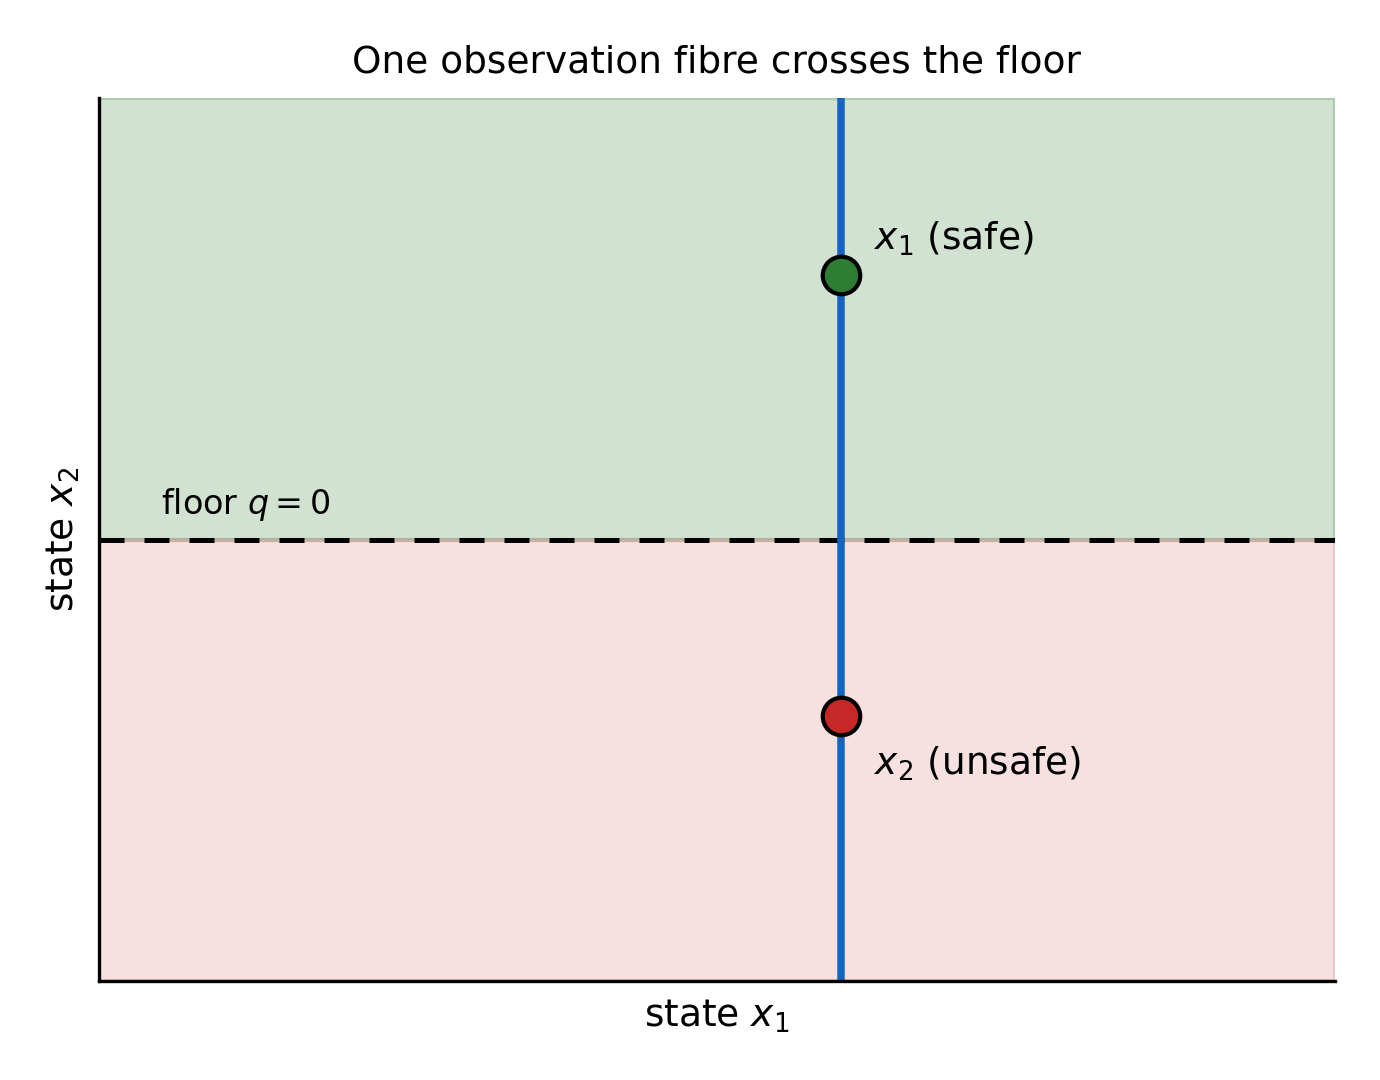
\includegraphics[width=0.82\columnwidth]{figs_p2/fig_p2_fibre.png}
\caption{An observation fibre crossing a floor boundary. The observation
\(O(x)=x_1\) cannot separate the safe state \((0.6,0.8)\) from the unsafe
state \((0.6,0.3)\) on the same fibre, so no exact observation-only
certifier exists (Proposition~\ref{prop:fibre}).}
\label{fig:fibre}
\end{figure}
\rule{0.5\linewidth}{0.5pt}

\bigskip
\noindent\textbf{Complete discussion of the degenerate (deterministic) limit: the worked instances and the audit-slice table (main text, Section 10).}
The deterministic-kernel deficit bound, attained:
The proposition's bound applies to the following finite models with
deterministic single-successor transitions, deterministic observations,
and \(B=\mathrm{supp}(b)\). It does not extend on the strength of
transition support alone to a fixed stochastic disturbance mixture:
a bad successor of arbitrarily small positive probability can produce
a smaller deficit. Under the stated deterministic-kernel assumptions,
the two worked instances attain the lower bound
\(1-V_k(b)\ge\min_{x\in B}b(x)\); no continuous-state limit is claimed.

\textbf{A worked instance (the two-floor conflict).} Read a finite-action restriction of the two-floor system of Section 3.4 as a finite POMDP: states \(x_{1}\) and \(x_{2}\) share one observation; take the two representative actions \(A=\{0,1\}\subset[0,1]\) (the same values follow with the full interval in a non-finite-action version); the one-step violation probability is \(p(x_{1}, u) = 1\) for \(u > 0.4\) and \(0\) otherwise, and \(p(x_{2}, u) = 1\) for \(u < 0.6\) and \(0\) otherwise; the prior is uniform, \(b_{0} = (1/2, 1/2)\). Then \(\sum_{x} b_{0}(x)\, p(x, u) \ge 1/2\) for every \(u\), so the chance-constrained proposition of the main text (Section 10) gives \(V_{k}(b_{0}) \le 1/2\) for all \(k \ge 1\), and the chance constraint \(\mathbb{P}_{b,\pi} \ge 1 - \varepsilon\) is infeasible for every \(\varepsilon < 1/2\). The bound is attained: \(V_{1}(b_{0}) = 1/2\) (each action sacrifices exactly one floor), and the surviving floor is thereafter kept safe by its own action, so \(V_{k}(b_{0}) = 1/2\) for all \(k\). At the degenerate limit this reads \(B_{0} = \{x_{1}, x_{2}\} \notin \mathcal{W}_{1}\) with \(V_{k}(b_{0}) = 1 - \min_{x \in B_{0}} b_{0}(x) = 1/2\), the bound of the proposition (main text, Section 10) --- the chance-constrained obstruction evaluated at its exact value.

\textbf{A worked instance (the delayed hidden regime on the audit grid).} This is a \emph{class-restricted} finite POMDP calculation, not a direct application of the unrestricted-policy equivalence in the deterministic-kernel proposition of the main text (Section 10). Read the audit system of Section 9 as a finite POMDP over the declared whole-window hold class: states \((z,\theta)\) with \(\theta \in \{-1,+1\}\), prior \(b_{0} = (\tfrac{1}{2}, \tfrac{1}{2})\) on the two regimes from \(z_{0}\), no observation before \(T_{\mathrm{obs}}\), exact regime revelation at \(T_{\mathrm{obs}}\), and blind-window actions restricted to the declared holds \(u \equiv \pm 1\). Define \(V^{\mathrm{hold}}_{k,T_{\mathrm{obs}}}(b_0)\) by maximizing survival over this whole-window hold class with regime-adapted continuation after revelation. This is not the unrestricted \(V_k\) of Section 10; it requires remembering the chosen hold action. Its values are exact: for \(k \le T_{\mathrm{obs}}\),
\[
V^{\mathrm{hold}}_{k,T_{\mathrm{obs}}}(b_{0}) \;=\; \tfrac{1}{2}\bigl(\mathbf{1}[z_{0} - k \ge 1] + \mathbf{1}[z_{0} + k \ge 1]\bigr),
\]
since a hold drives one branch down at unit rate; and for \(k > T_{\mathrm{obs}}\),
\(V^{\mathrm{hold}}_{k,T_{\mathrm{obs}}}(b_{0}) = \tfrac{1}{2}\bigl(1 + \mathbf{1}[z_{0} \ge 1 + T_{\mathrm{obs}}]\bigr)\), the revealed regime then held to growth. Three alignments follow. First, \(V^{\mathrm{hold}}_{1,T_{\mathrm{obs}}}(b_{0}) = 1\) exactly when \(z_{0} \ge 2\): the one-step certificate's silent region is exactly the region where the first blind step is safe. Second, \(V^{\mathrm{hold}}_{k,T_{\mathrm{obs}}}(b_{0}) = 1\) for every \(k\) exactly when \(z_{0} \ge 1 + T_{\mathrm{obs}}\): the belief-state value reproduces the audit's viability boundary, so on this grid the certificate partition and the separately class-restricted values agree cell by cell. Third, every hold-class deficit equals \(\tfrac{1}{2}=\min_x b_0(x)\): the declining branch is the lost mass. The same pathwise minimum-mass argument works with the recursion \emph{also restricted to holds}, but this is not an application of the main deterministic-kernel proposition to its unrestricted \(\mathcal W_k\); for \(z_0\ge2\), per-step alternation changes both the unrestricted viability verdict and \(V_k\). Table~\ref{tab:beliefV} tabulates the slice \(z_{0} \in \{1.5, 2, 2.5\}\); the verification script evaluates all 48 cells in exact rational arithmetic and regenerates the table verbatim. The class declaration is load-bearing here, as in clause (iv) of the class-declaration theorem of the main text (Section 10): over unrestricted time-varying blind policies the alternating sequence keeps both branches within \(z_{0} \pm 1\), so the unrestricted value equals \(1\) exactly on \(\{z_{0} \ge 2\}\) --- the cells the timing bound covers are exactly the cells where in-window adaptivity rescues the declared hold class.

\begin{table}[t]
\centering
\footnotesize
\begin{tabular}{@{}ccccccl@{}}
\toprule
\(z_{0}\) & \(T_{\mathrm{obs}}\) & \(V^{\mathrm{hold}}_{1}\) & \(V^{\mathrm{hold}}_{2}\) & \(V^{\mathrm{hold}}_{3}\) & audit verdict & covering certificate \\
\midrule
1.5 & 1 & \(\tfrac{1}{2}\) & \(\tfrac{1}{2}\) & \(\tfrac{1}{2}\) & \(\bullet\) & common-action \\
1.5 & 2 & \(\tfrac{1}{2}\) & \(\tfrac{1}{2}\) & \(\tfrac{1}{2}\) & \(\bullet\) & common-action \\
1.5 & 3 & \(\tfrac{1}{2}\) & \(\tfrac{1}{2}\) & \(\tfrac{1}{2}\) & \(\bullet\) & common-action \\
2.0 & 1 & \(1\) & \(1\) & \(1\) & \(\circ\) viable & --- \\
2.0 & 2 & \(1\) & \(\tfrac{1}{2}\) & \(\tfrac{1}{2}\) & \(\ast\) & timing bound \\
2.0 & 3 & \(1\) & \(\tfrac{1}{2}\) & \(\tfrac{1}{2}\) & \(\ast\) & timing bound \\
2.5 & 1 & \(1\) & \(1\) & \(1\) & \(\circ\) viable & --- \\
2.5 & 2 & \(1\) & \(\tfrac{1}{2}\) & \(\tfrac{1}{2}\) & \(\ast\) & timing bound \\
2.5 & 3 & \(1\) & \(\tfrac{1}{2}\) & \(\tfrac{1}{2}\) & \(\ast\) & timing bound \\
\bottomrule
\end{tabular}
\caption{Belief-state safety values \(V^{\mathrm{hold}}_{k,T_{\mathrm{obs}}}(b_{0})\) on the audit slice,
computed over the declared hold class (exact rational values; the script
regenerates all 48 cells). The hold-class deficit is \(\tfrac{1}{2}\) on every hold-class nonviable
cell (the class-relative pathwise bound), and the hold-class value is
\(1\) for every horizon exactly when \(z_0\ge1+T_{\mathrm{obs}}\).
This table is not the unrestricted value recursion of the main proposition.}
\label{tab:beliefV}
\end{table}
\rule{0.5\linewidth}{0.5pt}

\bigskip

\section*{S2. The sufficiency landscape (full)}

\subsection{5. The Sufficiency Landscape}\label{the-sufficiency-landscape-cited}

The sufficiency results against which the obstruction calculus is
defined are standard; they are stated here for contrast, and proofs
appear in the cited sources.

\textbf{(a) Veliov's output-feedback condition.} Veliov (1993) considers the same problem as Section 3 (a tube in the state space under incomplete and inexact measurement) and gives a sufficient condition for the
existence of an \emph{output-feedback regulation map}: a set-valued
feedback of the measurement under which all trajectories starting from
the graph of the tube remain in it. Under perfect measurement his
condition reduces to the classical viability condition (Haddad, 1981).
The complementarity with this paper is exact: Veliov's theorem certifies
existence; the obstruction calculus certifies nonexistence; a problem that satisfies neither requires a stronger observer or a finer observation structure.

\textbf{(b) The estimation-tube programme.} Cardaliaguet, Quincampoix,
and Saint-Pierre (2007) pass from imperfect information in the
measurement space to perfect information in an estimation space of
\emph{sets} of compatible states: the value functions of the two
problems coincide, and the estimation-space problem admits a
Dini-derivative characterization. The reduction is exact for value
functions; what it does not supply is a \emph{common prescription}. The exact relationship is stated in Section 6.3: carried out under the set-membership semantics, the estimation-space solution propagates the belief under a single control signal, so its controls \emph{are} common controls and joint admissibility is built into the estimation-space problem's own admissibility. Pointwise selections taken without that joint-admissibility check need not be jointly admissible; the common-action obstruction (Theorem~\ref{thm:common-action}) is the certificate that no jointly admissible selection exists at the information state in question.

\textbf{(c) Observer-and-buffer transfer.} A full-information feedback \(k(x)\) and an observer estimate \(\hat x\) alone do not prove invariance. If a specified compact set \(K_\zeta\) has been proved invariant under every \emph{admissible} input perturbation \(u=k(x)+v\) with \(\|v\|\le\rho\), then using \(k(\hat x)+\delta u\) inherits that guarantee whenever
\[L_k\|\hat x(t)-x(t)\|+\|\delta u(t)\|\le\rho\]
for all relevant times and the implemented command remains admissible. An exponentially decaying observer bound may imply this inequality from a sufficiently small initial error, but the robust-input radius \(\rho\), the admissibility condition and the invariant set must be established for the particular plant; no universal erosion coefficient or no-loss theorem is asserted here.

\textbf{(d) The linear substitution alternative.} Let \(a\in\mathbb R^k_{\ge0}\) be pathways with constraints \(Ra\le x\), \(Ea\le e\), and \(Qa\ge s^{\mathrm{req}}\), where \(R\in\mathbb R^{n\times k}\), \(E\in\mathbb R^{m\times k}\), \(Q\in\mathbb R^{p\times k}\), and \(x,e,s^{\mathrm{req}}\) have matching dimensions. For this specified finite linear model, exactly one of the following holds
(Farkas, 1902; Gale, 1960): (i) there exists a non-negative pathway
vector \(a \ge 0\) satisfying the linear substitution constraints; or
(ii) there exist multipliers \(\alpha, \beta, \gamma \ge 0\) such that
\[\alpha^\top R + \beta^\top E - \gamma^\top Q \ge 0 \quad\text{componentwise},\qquad \gamma^\top s^{\mathrm{req}} > \alpha^\top x + \beta^\top e.\]
The second statement is a certificate that the specified substitution pathways cannot meet demand within the typed resource and capacity
bounds; writing all constraints as \(Aa \le \rho\), the pair is the Farkas lemma alternative. The multipliers are a separation
certificate, not universal exchange rates: nonlinear, nonconvex,
path-dependent, spatial, or irreversible technologies require their own
feasibility analysis, and an elasticity fitted near one operating point
cannot establish global substitutability. This is the feasibility-side
complement of the observation-side obstructions of Sections 3--4: where
the present paper's certificates bound what \emph{information} can
achieve, the substitution alternative bounds what \emph{material
pathways} can achieve, and the same infeasibility logic --- exhibit the separating multiplier rather than assert impossibility --- applies to both.

\textbf{A worked comparison: barrier, estimation-tube, and obstruction certificates on one system.} The two-floor system of Section 3.4 makes the division of labour concrete. Two states \(x_1\) and \(x_2\) share one observation; the single control \(u\in[0,1]\) must satisfy \(u\le 0.4\) at \(x_1\) (floor 1 active) and \(u\ge 0.6\) at \(x_2\) (floor 2 active).

\emph{Barrier certificates.} A state-dependent barrier need not be constant on an observation fibre merely because the controller is output-based. What fails in this two-state instance is the existence of a \emph{common safe action} satisfying the incompatible floor inequalities at both states; a search restricted to observation-only barriers may be inconclusive about more general barrier methods. Any theorem transferring a particular barrier construction or estimation-space value to this model requires matching its primary-source hypotheses. No general nonexistence of a state-dependent barrier is inferred solely from a fibre-constancy argument.

\emph{Estimation-tube reduction.} Lifting to the estimation space replaces the merged observation by perfect information about the belief \(\{x_1,x_2\}\). The belief-state viability problem then has empty value --- no common control keeps both floors safe --- so the estimation-space kernel is empty. Where the cited estimation-space reduction applies with matching policy and admissibility hypotheses, it returns the verdict; without those hypotheses the reduction is not a separate proof. In that setting, the value alone does not isolate the cause: it does not isolate which feature of the observation is responsible.

\emph{Obstruction certificate.} The common-action obstruction (Theorem~\ref{thm:common-action}) fires with the explicit Farkas certificate \(\lambda=(1/2,1/2)\) for the stacked system \(u\le 0.4\), \(-u\le -0.6\), with \(\lambda^{\top}A=0\) and \(\lambda^{\top}b=-0.1<0\) --- the infeasibility margin \(0.1\) of Section 3.4. The sparse witness of Section 3.4 records that \(m+1=2\) states already suffice, and the certificate licenses a concrete remedy: any observation separating \(x_1\) from \(x_2\) restores one-step viability. (The general polyhedral statement and its checkability discussion are the complete-discussion block of S1.) This is the division of labour the paper relies on --- the estimation-tube reduction returns the empty-kernel verdict; the obstruction calculus certifies \emph{why} with a checkable witness and names the observation feature to change. The unsuccessful search for a barrier is inconclusive on emptiness.


\begin{center}\rule{0.5\linewidth}{0.5pt}\end{center}


\bigskip
\noindent\textbf{Complete proof of the linear-programming instantiation theorem (main text,
Section 3.3).} Unroll the affine dynamics: for step \(k\),
\[
x_{j,k} \;=\; A_{j}^{\,k} x_{j,0} \;+\; \sum_{i=0}^{k-1} A_{j}^{\,k-1-i}\bigl(B_{j} u_{i} + E_{j} w_{j,i}\bigr),
\qquad w_{j,i} \in W_{j}.
\]
For every branch \(j\), step \(k\), and floor row \(r\), the robust inequality \(F_r x_{j,k}\le g_r\) for all \emph{independently selectable} disturbances \(w_{j,t}\in W_j\) is equivalent to
\[\sum_{t=0}^{k-1}F_r A_j^{k-1-t}B_j u_t
\le g_r-F_r A_j^k x_{j,0}-\sum_{t=0}^{k-1}h_{W_j}\!\left(E_j^{\top}(A_j^{k-1-t})^{\top}F_r^{\top}\right).\]
The row index \(r\) is not the disturbance-time index \(t\). With coupled disturbance paths, the sum of independent support values must be replaced by the support of the joint admissible path set.
where \(h_{W_{j}}\) is the support function of \(W_{j}\); each support value is itself a
linear program over the polytope \(W_{j}\), precomputed once, exactly in rational
arithmetic. The horizon-\(K'\) feasibility program is therefore
\(\{G u \le b\}\) in the variables \(u_{0},\dots,u_{K'-1}\), with one row per (branch, step,
floor constraint) and the box rows of \(U\); its size is polynomial in \(K'\), \(|J|\), and
the description lengths. Feasibility is monotone in \(K'\) because the rows of a shorter
horizon are a subset of those of a longer one, so \(\sigma^{*}(B_{0};\Pi_{B}) = \max\{K'
\le K : \text{feasible}\}\) is computable by bisection with \(\lceil \log_{2} K \rceil + 1\)
programs: claim (i). Claim (ii) is Farkas' lemma: infeasibility of \(\{Gu \le b\}\) yields
\(\lambda \ge 0\) with \(\lambda^{\top} G = 0\) and \(\lambda^{\top} b < 0\); indexing
\(\lambda\) by (branch, step, constraint) gives nonnegative adjoint rows whose aggregate
control projection vanishes and whose aggregate constant is negative. Claim (iii) is
definitional: the program's feasible set is, by construction,
\(\{(u_{0},\dots,u_{K-1}) \in \Pi_{B} : \text{every branch in } \mathcal{V} \text{ through
step } K\}\), so no relaxation is taken and the computation is sound and complete over the
declared class.

For claim (iv), \emph{two distinct systems} are checked.
\emph{Hidden-regime hold-versus-relaxation gap:} with branches
\(z^{+}=z+u\), \(z^{-}=z-u\), floor \(z\ge1\), declare
\(\Pi_{\mathrm{hold}}=\{(u,\ldots,u):u\in\{\pm1\}\}\) over the
entire blind window. At \(z_0=2\), either hold keeps both branches
safe for exactly one step, then one exits on step two. The polytope
per-step relaxation \(u_k\in[-1,1]\) admits \(u\equiv0\), which keeps
both branches at \(z_0\) through every horizon. Thus the difference
in maximal safe-step counts grows without bound as \(K\) increases.
This comparison is \emph{not} between all finite per-step sequences
\(u_k\in\{\pm1\}\) and the polytope: in that larger finite class,
alternation can keep both branches safe from \(z_0=2\).
For general real \(z_0\ge1\), a whole-window hold survives
\(\lfloor z_0-1\rfloor\) integer blind steps, with the real quantity
\(z_0-1\) marking its linearly interpolated floor-crossing time.
\emph{Decaying-system duality computation (a separate model):} with branches \(z^{+} = \tfrac{9}{10} z \pm u\), the
level-\(k\) rows are \(z^{+}_{k} \ge 1\) and \(z^{-}_{k} \ge 1\) with
\(z^{\pm}_{k} = (\tfrac{9}{10})^{k} z_{0} \pm \sum_{i<k} (\tfrac{9}{10})^{k-1-i} u_{i}\).
Summing the pair cancels the control terms pairwise (equal magnitudes, opposite signs),
leaving \(2 (\tfrac{9}{10})^{k} z_{0} \ge 2\): a Farkas combination proving
\(z_{0} \ge (\tfrac{10}{9})^{k}\), with the vanishing aggregate control projection visible
as the pairwise cancellation. Necessity also follows control-independently from the branch
sum \(z^{+}_{k} + z^{-}_{k} = 2 (\tfrac{9}{10})^{k} z_{0}\); sufficiency at the boundary
\(z_{0} = (\tfrac{10}{9})^{K}\) is witnessed by \(u \equiv 0\), which keeps the branches
balanced at \((\tfrac{10}{9})^{K-k} \ge 1\). The threshold is therefore exact, and the
program is a complete characterization of the declared class. All twelve computations in
this proof and the next are machine-verified in exact rational arithmetic (fractions, no
floating point): the survival-time identity and the \(42 = 30 + 12\) audit partition of the
hidden-regime grid; the extinguishing of the certificate under the polytope relaxation; the
level-\(k\) pairwise cancellations and deepest bound for \(K \le 3\); the boundary control;
and the four-state computations below.
\rule{0.5\linewidth}{0.5pt}

\bigskip
\noindent\textbf{Two-phase policy decomposition (main article, Section 7).} A viable policy restricts to one blind control that keeps \emph{every} compatible trajectory safe through the window. For each possible terminal observation, its continuation must be viable from that terminal information state. Under full physical-state revelation the terminal condition is membership of each terminal state in the matched full-information state kernel; under branch-only revelation with residual within-branch uncertainty, it is membership of each branch-conditional \emph{belief} in the post-reveal epistemic kernel. Conversely, if one blind command sequence satisfies both window safety and the relevant terminal condition, and the declared policy class admits nonanticipative pasting of the terminal strategies, concatenate those continuations to obtain a viable policy. This is not a claim that silence of an incomplete window certificate proves viability or that branch revelation automatically reveals the physical state.
\rule{0.5\linewidth}{0.5pt}

\bigskip
\noindent\textbf{Complete proof of the window-measurability no-go (main text, Section 7).}
The instance of Supplementary S3/A.3 has states \(x_{1}, x_{2}, x_{3}, x_{4}\) with safe
set \(\{x_{1}, x_{2}, x_{4}\}\), transitions \(x_{1}\): \(a \to x_{1}\), \(b \to x_{4}\);
\(x_{2}\): \(a \to x_{4}\), \(b \to x_{2}\); \(x_{4}\): \(a \to x_{3}\), \(b \to x_{3}\);
initial belief \(B_{0} = \{x_{1}, x_{2}\}\), blind at the first step and exactly informed
after. The variant changes only \(x_{4}\)'s post-reveal transitions to
\(a \to x_{4}\), \(b \to x_{4}\). All window sub-model data coincide: the same \(B_{0}\),
the same first-step transitions of \(x_{1}\) and \(x_{2}\), the same floor, the same
schedule. Both certificates are silent in each: each blind action keeps both branches in
the safe set through the window step, so the common-action and timing certificates have no
witness. The exact recursion decides differently. In the instance, every post-reveal action
from \(x_{4}\) exits the safe set, so \(x_{4} \notin \mathrm{RViab}(\mathcal{V})\), the
one-step-backward pass misses \(B_{0}\) at horizon two, and \(B_{0}\) is nonviable; in the
variant, \(x_{4}\) is maintained under both actions, \(x_{4} \in
\mathrm{RViab}(\mathcal{V})\), the action \(a\) lands \(x_{1}\) and \(x_{4}\) in the
kernel, and \(B_{0}\) is viable. Any window-measurable pair returns identical verdicts on
the two instances, so no window-measurable pair is complete. The verification record
confirms each step in exact arithmetic: certificate silence in both instances; nonviability
of the instance at horizon two with failure exactly on clause (ii) of the decomposition
(every window-surviving blind action lands a branch outside the kernel); and viability of
the variant.

\section*{S3. Bounded constructions and scope remarks}

\subsection{Appendix A: Bounded Constructions and Scope
Remarks}\label{appendix-a-bounded-constructions-and-scope-remarks}

The bounded constructions below complement the obstruction theorems of Sections 3--4. They are stated in full, together with their scope remarks.

\textbf{A.1 Example (coupling creates viability absent in a factor).}
Take the two-patch logistic system
\(\dot S_i = g_i(S_i) + \kappa\,(S_j - S_i) - h_i, \qquad i, j \in \{1,2\},\ i \ne j,\)
with \(g_i(s) = s(1-s)\), \(\kappa = 0.2\), constraints \(S_i \in [0,1]\) and \(h_i \ge h_{\min,i}\) (harvest floors), and admissible controls the constant harvest vectors \(h = (h_1, h_2)\) with \(h_i \ge 0\). Choose
\((S_1^*, S_2^*) = (0.5, 0.8)\). Define harvest floors by the equilibrium equations: \(h_{\min,1} = g_1(0.5) + 0.2(0.8 - 0.5) = 0.31\); \(h_{\min,2} = g_2(0.8) + 0.2(0.5 - 0.8) = 0.10\). Patch 1 in isolation:
\(\max_s g_1(s) = 0.25 < h_{\min,1} = 0.31\), so patch 1 is not viable
in isolation. Yet the coupled system has the equilibrium \((0.5, 0.8)\)
with \(h = (0.31, 0.10)\) admissible and the stock constraints
satisfied, so its kernel is nonempty. The example is the constructive
counterpart of the emptiness results of Section 3: where the obstruction
theorems certify that no policy works for reasons of information, patch
coupling exhibits the opposite direction --- a jointly viable operating
point that no factor sustains alone.

\textbf{A.2 Counterexample (emptiness despite factorwise viability at
MSY).} Take \(\kappa > 0\), \(C_1 \ne C_2\), \(h_{\min,i} = r_i C_i / 4\) (MSY level), in the same coupled system with \(\phi_i(S_i) := g_i(S_i) - h_{\min,i}\) and growth laws
\(g_i(S) = r_i S (1 - S/C_i)\), so that
\[\phi_i(S_i) = -\frac{r_i}{C_i}\left(S_i - \frac{C_i}{2}\right)^2 \le 0\]
with equality only at \(S_i = C_i/2\), and the constraint set is the compact box \([C_1/2, \bar S_1] \times [C_2/2, \bar S_2]\) with fixed finite \(\bar S_i>C_i/2\). The admissible harvests in this construction are time-constant \(h_i\ge h_{\min,i}\). Each isolated system has kernel \([C_i/2, \bar S_i]\) (from \(S_i > C_i/2\) the stock
declines toward \(C_i/2\) asymptotically, never below). For the coupled
system, define the Lyapunov function \(W = S_1 + S_2\); then
\[\dot W = \phi_1(S_1) + \phi_2(S_2) \le 0,\] with equality exactly at
\(p^* = (C_1/2, C_2/2)\), where the flow is nevertheless nonzero:
\(\big(\dot S_1, \dot S_2\big)\big|_{p^*} = \left(\tfrac{\kappa}{2}(C_2 - C_1), \tfrac{\kappa}{2}(C_1 - C_2)\right) \ne 0.\)
Suppose a trajectory remained in the constraint box for all time. Then
\(W\) is non-increasing and bounded below by \((C_1 + C_2)/2\), so
\(W(t) \downarrow W_\infty \ge (C_1 + C_2)/2\); the \(\omega\)-limit set
of the trajectory is nonempty, compact, and invariant, and
\(\dot W \equiv 0\) on it (otherwise \(W\) would keep decreasing along
the set). Hence the \(\omega\)-limit set is contained in \(\{p^*\}\), so
it equals \(\{p^*\}\) and the trajectory converges to \(p^*\). But a singleton \(\omega\)-limit set of an autonomous smooth flow is invariant only if its point is an equilibrium. Since \(f(p^*)\ne0\), no nonempty invariant subset of \(\{p^*\}\) exists. For any time-constant harvest strictly exceeding the minimum in at least one coordinate, \(\dot W\le-\sum_i(h_i-h_{\min,i})<0\) gives the contradiction directly from the lower bound on \(W\). The argument for the minimum-harvest equality case is the compact invariant-set contradiction just proved. A separate proof is needed for any time-varying harvest class.
Therefore, in the declared constant-harvest class, no trajectory remains in the compact box for all time: its restricted kernel is empty, and every such trajectory violates a constraint in finite time. Note the logical
order: the emptiness conclusion here rests on the
Lyapunov--\(\omega\)-limit argument, \emph{not} on the absence of an
equilibrium --- absence of equilibria alone does not imply an empty
kernel (periodic and nonstationary viable trajectories are possible in
general), and the two are kept separate. The counterexample is
specific to the MSY parameter choice; for \(H_{\min,i} < r_i C_i / 4\),
equilibria may exist. Together with A.1 it delimits what coupling can
and cannot repair: factorwise nonviability is repairable (A.1), but
factorwise viability at an incompatible operating point is not (A.2).

\textbf{A.3 Example (insufficient post-observation recourse).} A four-state system (three safe states) shows the mode of Section 6.5(ii) concretely. Take \(\mathcal{V} = \{x_{1}, x_{2}, x_{4}\}\) with \(x_{3} \notin \mathcal{V}\) a violation, actions \(A = \{a, b\}\), and no disturbance. Transitions: \(x_{1}\) maps to \(x_{1}\) under \(a\) and to \(x_{4}\) under \(b\); \(x_{2}\) maps to \(x_{4}\) under \(a\) and to \(x_{2}\) under \(b\); \(x_{4}\) maps to \(x_{3}\) under both actions, so \(x_{4}\) lies in \(\mathcal{V}\) but outside the kernel. The observation merges \(x_{1}\) and \(x_{2}\) at the first step and is exact thereafter. The root belief \(B_{0} = \{x_{1}, x_{2}\}\) is one-step viable: action \(a\) keeps both states in \(\mathcal{V}\) (reaching \(x_{1}\) and \(x_{4}\)), as does \(b\) (reaching \(x_{4}\) and \(x_{2}\)), so the common-action certificate is silent and no exit occurs in the first step. After the first observation, however, the trajectory is at \(x_{4}\) for one of the two possible initial states (under \(a\) it is \(x_{2}\), under \(b\) it is \(x_{1}\)), and \(x_{4}\) has no safe action, so that branch exits at the second step regardless of what the policy learns. Hence \(B_{0} \notin \mathcal{W}_{2}\) although \(B_{0} \in \mathcal{W}_{1}\): the failure is a post-observation recourse failure, witnessed only by the recursion (Theorem~\ref{thm:finite-horizon}) --- the exit certificate is silent at the root because both \(x_{1}\) and \(x_{2}\) are individually viable under full information, and the timing certificate is silent because the observation arrives without delay. The main text supplies the continuous-time counterpart (Section 3.7 there): an oracle-relaxed recourse obstruction whose three-branch braking instance fires exactly in this regime --- blind-window safety with insufficient post-observation braking authority --- with exact delay threshold \(\tau = 7/50\).


\renewcommand{\thefigure}{S\arabic{figure}}%
\setcounter{figure}{0}%

\section*{S4. Additional figures}

\begin{figure}[htbp]
\centering
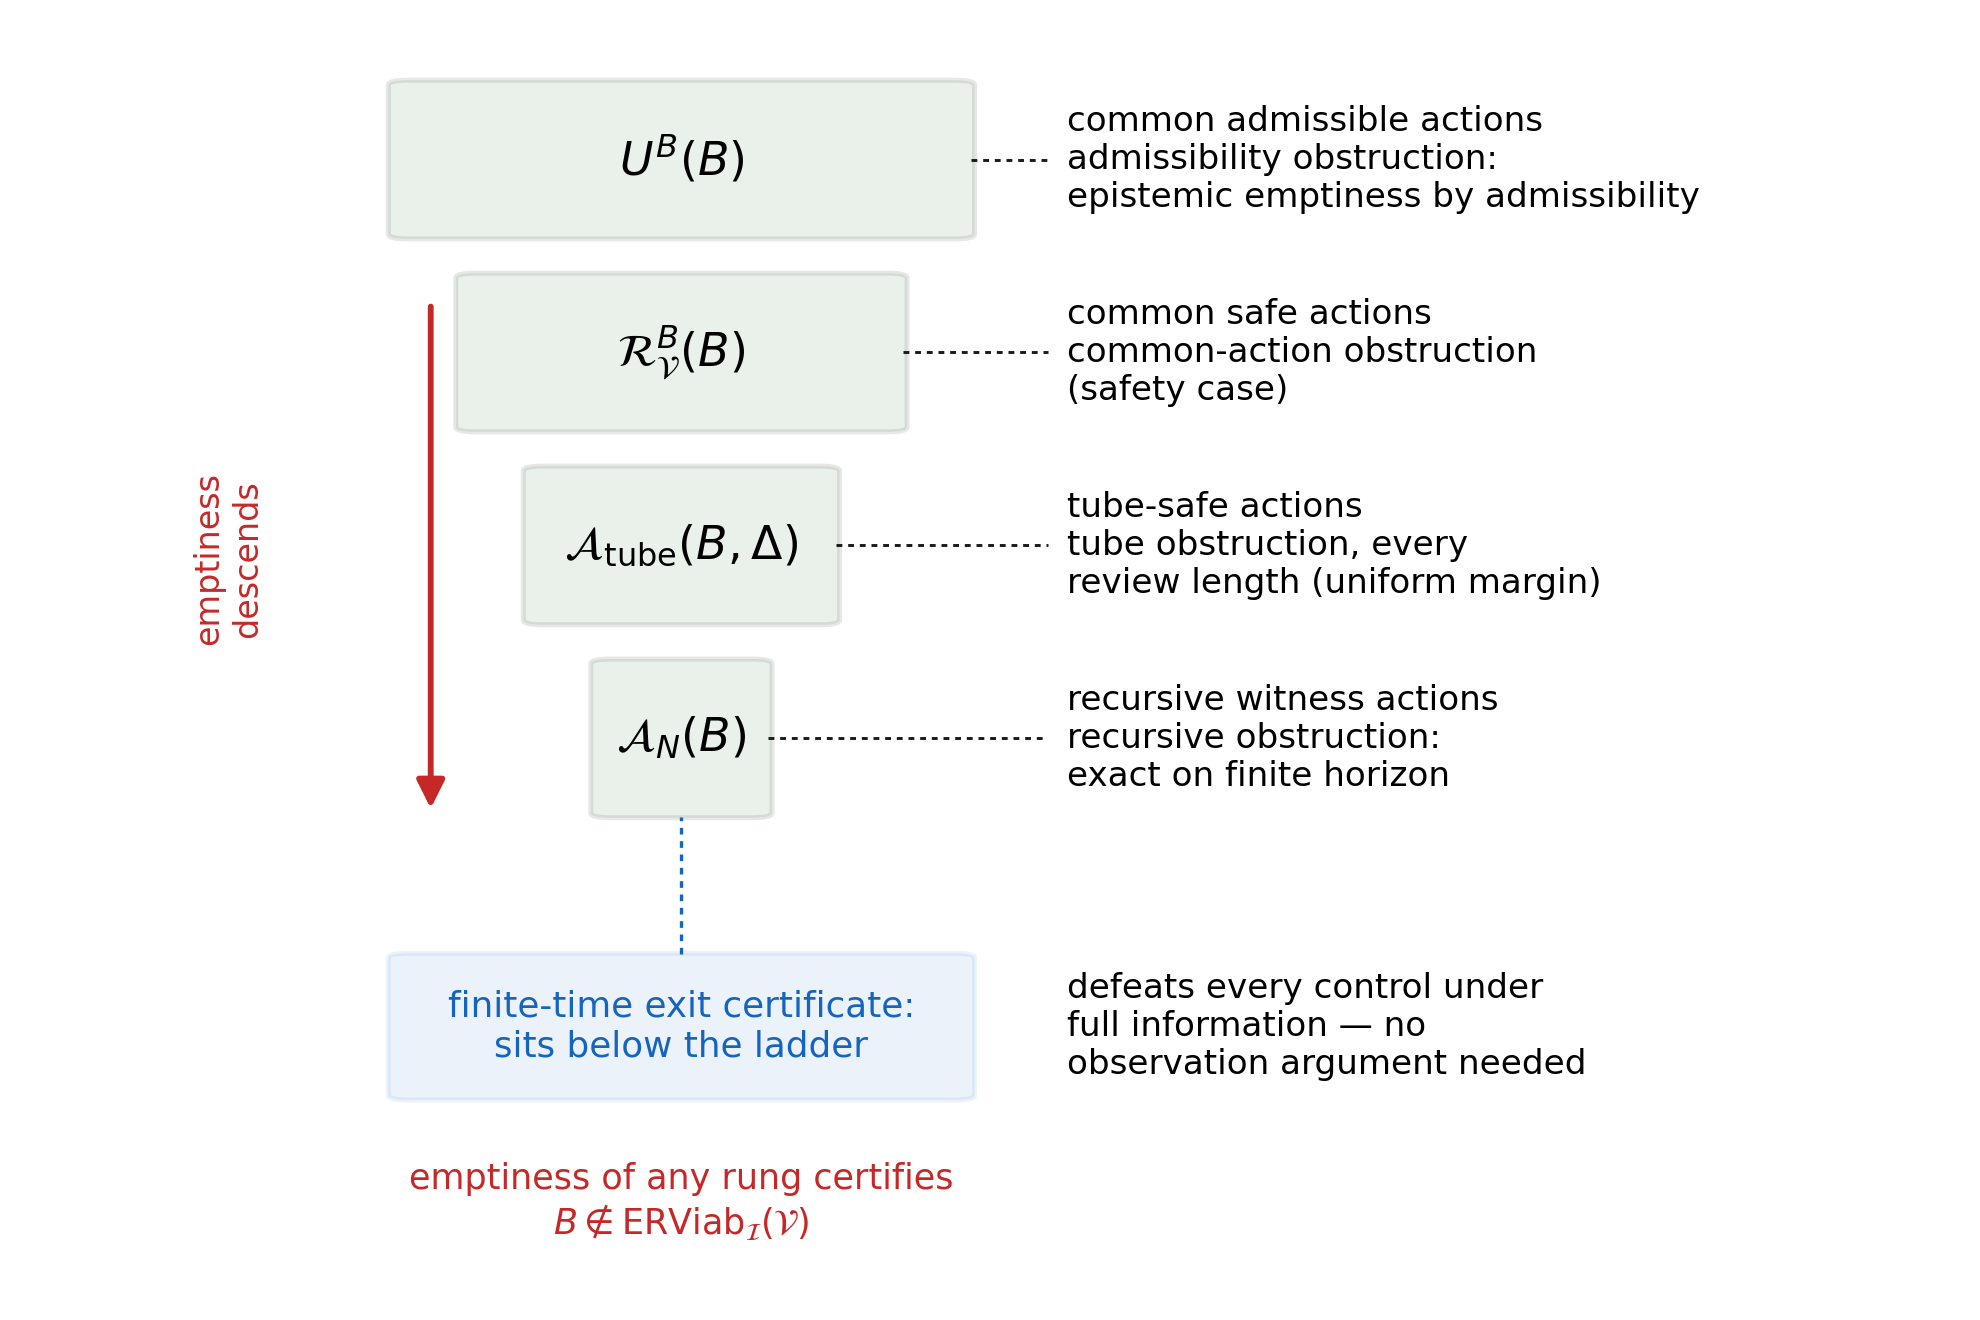
\includegraphics[width=0.75\linewidth]{figs_p2/fig_p2_ladder.png}
\caption{The obstruction ladder. The common response sets form nested necessary
conditions for viability,
\(U^B(B)\supseteq\mathcal{R}_{\mathcal{V}}^B(B)\supseteq\mathcal{A}_{\mathrm{tube}}(B,\Delta)\); the discrete \(\mathcal A_N\) needs a sampled model bridge,
and emptiness descends (Proposition~\ref{prop:ladder}); the finite-time
exit certificate sits below the ladder, defeating every control under
full information (Theorem~\ref{thm:exit}).}
\label{fig:ladder}
\end{figure}

\begin{figure}[htbp]
\centering
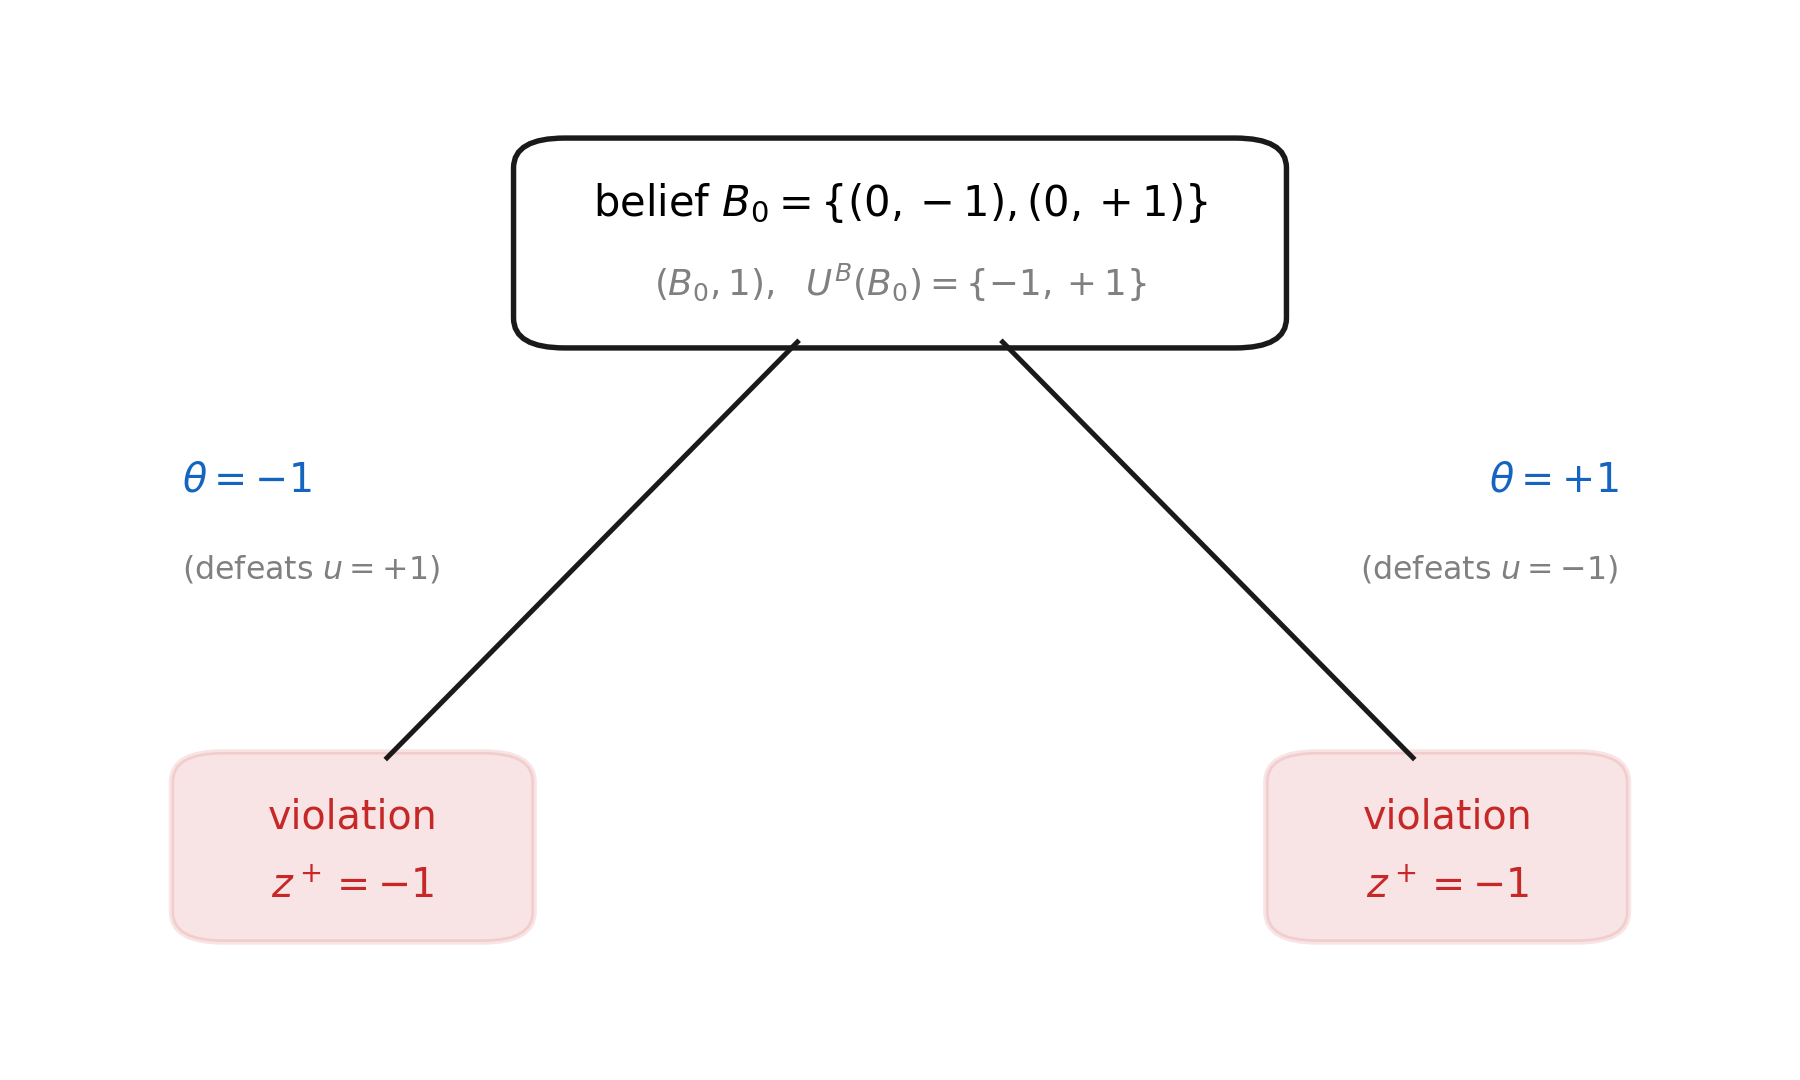
\includegraphics[width=0.66\linewidth]{figs_p2/fig_p2_obstruction_tree.png}
\caption{The one-step obstruction tree of Example~\ref{ex:hidden-mode},
read as a finite system: for each admissible action the adversary has a
compatible branch terminating in violation, so \(B_0\notin\mathcal{W}_1\)
(Theorem~\ref{thm:finite-horizon}).}
\label{fig:obstruction-tree}
\end{figure}

\begin{figure}[htbp]
\centering
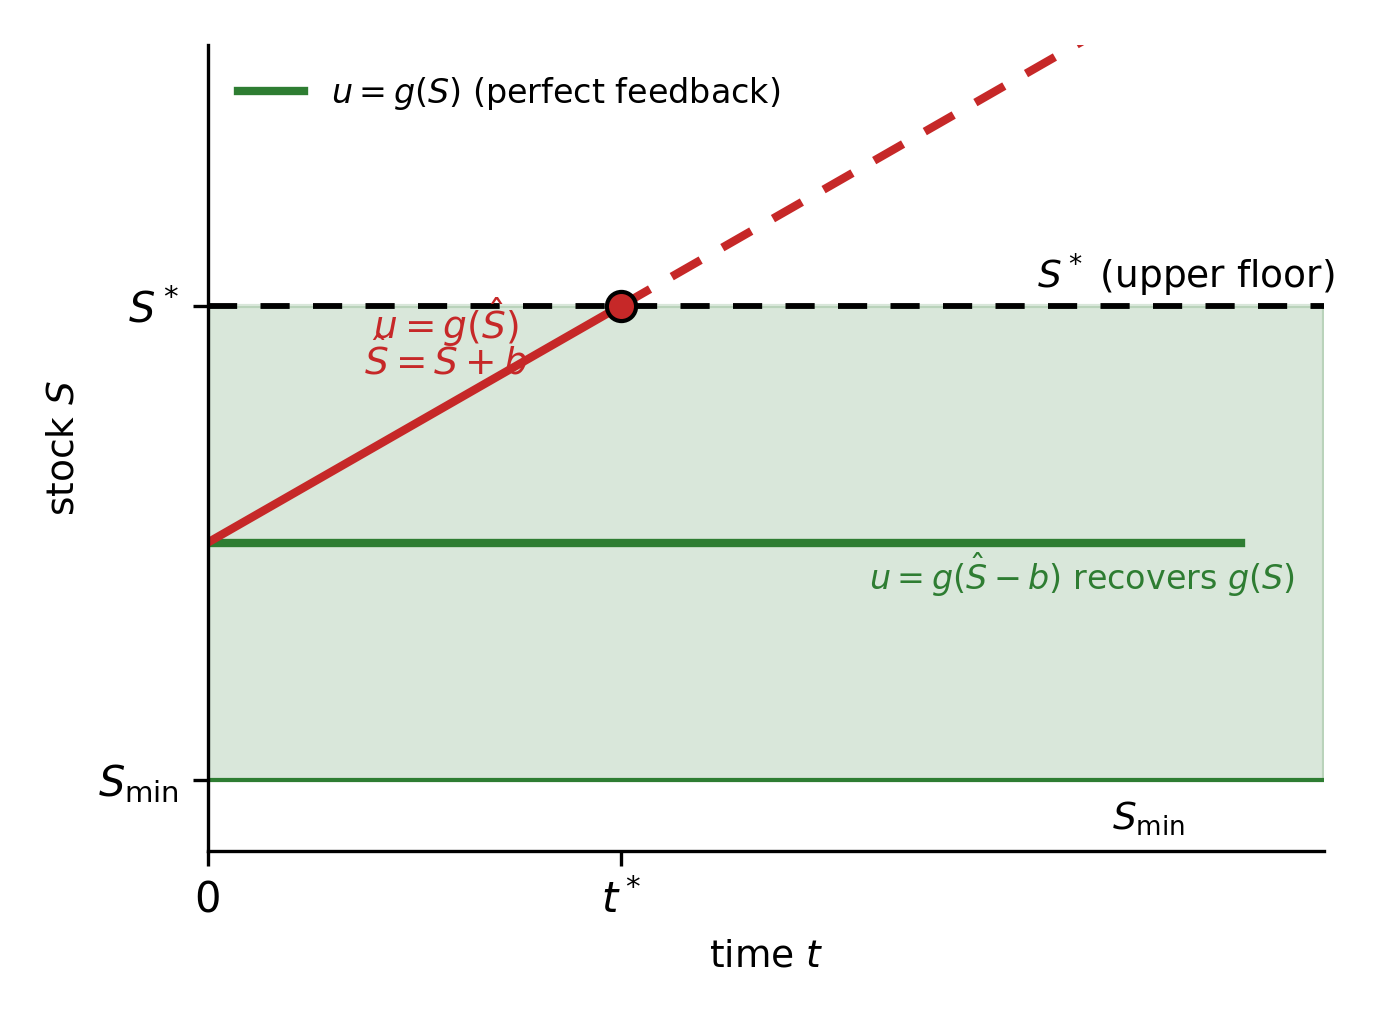
\includegraphics[width=0.62\linewidth]{figs_p2/fig_p2_ce_trap.png}
\caption{The certainty-equivalence trap. Under the perfect-information
law \(u=g(S)\) the stock is stationary inside \(\mathcal V\). Applying
the same law to the biased observation \(u=g(\hat S)\) with
\(\hat S=S+b\) gives \(\dot S=g(S+b)-g(S)>0\), so \(S\) exits above
\(S^*\) in finite time (Remark~\ref{rem:ce-trap}); inverting the bias
restores \(g(S)\).}
\label{fig:ce-trap}
\end{figure}

\section*{Auxiliary definitions and remarks (for reference)}

\begin{definition}[robust epistemic kernel]\label{def:kernel}

\(B_0 \in \mathrm{ERViab}_{\mathcal{I}}(\mathcal{V})\) if there exists a
nonanticipative observation-based policy \(\pi\) such that, for every
compatible initial state \(x_0 \in B_0\) and every admissible
disturbance realization \(d(\cdot)\), the trajectory of
\(\dot x = f(x, u(t), d(t))\) generated from \(x_0\) by \(\pi\)'s
actions under \(d(\cdot)\) --- the record being the one that
\((\pi, d(\cdot))\) generates --- remains in \(\mathcal{V}\) for all
time. (This is the standard exists-strategy-for-all-realizations form. The quantifier order is essential: the record is generated by the realization, so conditioning the admissible realizations on the record would be circular.) The common ambient prior domain is \(\mathfrak B=\{B\subseteq X:B\ne\varnothing\}\), matching the main article. The initial observation splits a prior \(P\) into nonempty post-observation cells \(P\cap O^{-1}(y)\). A singleton prior remains singleton under a constant observation, and compactness is imposed separately in statements that need it. The existential (non-robust) counterpart \(\mathrm{EViab}_{\mathcal{I}}(\mathcal{V})\) is the non-robust contrast class.

\end{definition}

\begin{proposition}[selector principle]\label{prop:selector}
If \(B\in\mathrm{ERViab}_{\mathcal{I}}(\mathcal{V})\) and \(\pi\) is a
policy witnessing viability on \(B\), then at every review time the
action \(a=\pi(B)\) selected by \(\pi\) is a response that is
(i) \emph{admissible}, \(a\in U^B(B)\); (ii) \emph{safe}, keeping every
compatible trajectory in \(\mathcal{V}\) until the next observation ---
\(\mathrm{Reach}_{[0,\Delta]}(B,a)\subseteq\mathcal{V}\) at review
length \(\Delta\); and (iii) \emph{recursively viable}, in that every
post-observation belief reached at the next review is again in
\(\mathrm{ERViab}_{\mathcal{I}}(\mathcal{V})\) under the continuation
of \(\pi\). A belief is therefore viable only if each of the response
correspondences of this section --- \(U^B(B)\),
\(\mathcal{R}_{\mathcal{V}}^B(B)\), \(\mathcal{A}_{\mathrm{tube}}(B,\Delta)\),
and the recursive predecessor of Section 3.1 --- is nonempty along
every reachable branch; hence a certificate that any one of them is
empty at a reachable belief certifies nonviability. In finite systems
the converse is exact (Theorem~\ref{thm:finite-horizon}); in continuous time a converse for unrestricted policies is not established by the finite recursion, and remains open under the stated class and observation assumptions (main article, Section 7).
\end{proposition}

\begin{remark}[comparison-function form]\label{rem:comparison}
Suppose a compatible original-system adverse path satisfies \(\dot q\le-\alpha(q)\) while \(q>0\), with \(\alpha(s)>0\) on \((0,a]\). A finite comparison integral \(\int_0^{q(x_0)}ds/\alpha(s)\) bounds \emph{first contact}, not necessarily strict exit from the closed safe set. For example \(\dot q=-\sqrt q\), \(q(0)=1\), reaches zero at time two and may remain there. Strict exit additionally needs compatible continuation with adverse drift at or through boundary contact; a formal value \(\alpha(0)>0\) without such a path is insufficient.
\end{remark}

\begin{example}[hidden-mode conflict]\label{ex:hidden-mode} Let an unobserved parameter satisfy
\(\theta \in \{-1, +1\}\), with \(\dot z = \theta u\),
\(u \in \{-1, +1\}\), and constraint \(z \ge 0\). At \(z = 0\): if
\(\theta = +1\), only \(u = +1\) is safe; if \(\theta = -1\), only
\(u = -1\) is safe. Both compatible states are individually robustly
viable under full information (each admits its safe control), but the
information set \(B = \{(0, +1), (0, -1)\}\) satisfies
\(\mathcal{R}_{\mathcal{V}}^B(B) = \{+1\} \cap \{-1\} = \varnothing\),
so \(B \notin \mathrm{ERViab}_{\mathcal{I}}(\mathcal{V})\). This is a
purely informational failure: no stochasticity and no estimation-quality
argument is involved. The example is the two-action skeleton of every
``the stock is either recovering or collapsing, and the safe policy
differs between the two'' situation.

\end{example}

\begin{remark}[threshold form of the timing obstruction]\label{rem:sigma}
For a declared blind-window policy class \(\Pi\), define the
class-relative guaranteed survival time by
\[\sigma^*_{\Pi}(B_0)=\sup_{u(\cdot)\in\Pi}
\inf_{x_0\in B_0,\,d(\cdot)}\tau(x_0,u,d),\]
where the infimum ranges over observation-equivalent branches and
\(\tau\) is the first strict violation time. Then
\[\sigma^*_{\Pi}(B_0)<T_{\mathrm{obs}}\ \Longrightarrow\
\text{no policy in }\Pi\text{ is viable from }B_0.\]
Only for the unrestricted class is this an assertion that
\(B_0\notin\mathrm{ERViab}_{\mathcal I}(\mathcal V)\).
Before the first observation a policy cannot distinguish branches.
Under (H3.1)--(H3.2), for \emph{every} control in \(\Pi\) at least
one compatible branch exits by time
\(\inf_{x\in B_0}q(x)/\varepsilon\), hence
\(\sigma^*_{\Pi}(B_0)\le\inf_{x\in B_0}q(x)/\varepsilon\), and (3) states that
this upper bound lies below \(T_{\mathrm{obs}}\); the threshold itself
may be strictly smaller, in which case nonviability holds even when (3)
fails. The threshold is the blind-window response correspondence of the
timing layer: its emptiness is the timing certificate, the
delayed-information analogue of the tube and common-action
correspondences.
\end{remark}

\begin{definition}[exact certifier]\label{def:certifier}

For an admissible domain
\(Z \subseteq X\) and a safe set \(K \subseteq Z\), an \textbf{exact
certifier} based on the observation map \(O : Z \to Y\) is a function
\(C : Y \to \{0,1\}\) such that
\[C(O(z)) = 1 \iff z \in K \qquad \text{for every } z \in Z.\]

\end{definition}

\begin{remark}[the certainty-equivalence trap]\label{rem:ce-trap}

Consider \(\dot S = u - g(S)\) with \(u \in [0, \bar u]\), \(g\) continuous and strictly
increasing on \([S_{\min}, S^* + b]\), \(g(0) = 0\), and
\(\mathcal{V} = [S_{\min}, S^*]\). Assume the range condition
\(g(S + b) \le \bar u\) for every \(S \in [S_{\min}, S^*]\), so that the
controller below is admissible. Under perfect information the zeroing
feedback \(u(t) = g(S(t))\) gives \(\dot S = 0\), so every
\(S_0 \in \mathcal{V}\) is viable and
\(\mathrm{Viab}(\mathcal{V}; U, \pi_{\mathrm{perf}}) = \mathcal{V} \neq \varnothing\).
Now take the injective, biased observation \(\hat S = S + b\) with
\(b > 0\), and the canonical certainty-equivalence controller: the
perfect-information zeroing law applied directly to the uncorrected
observation, \(u = g(\hat S) = g(S + b)\). Then
\[\dot S = g(S + b) - g(S) > 0 \qquad \forall S,\]
and since \(g\) is strictly increasing on the compact interval
\([S_{\min}, S^* + b]\), \(\dot S\) is bounded below by a positive
constant there; hence \(S\) strictly increases and exits above \(S^*\) in
finite time from every \(S_0 \in \mathcal{V}\): the kernel of this single
controller is empty. The bias-corrected controller
\(u = g(\hat S - b) = g(S)\) uses the observation map's structure, restores
\(\dot S = 0\), and keeps the kernel nonempty.

The mechanism is a \emph{failure of one policy to use the observation
map's structure}, not a loss of information: for a known invertible
observation the output-feedback class is as powerful as the
state-feedback class. No analogy to signalling or nonclassical information is required for this known-bias example. The remark is
policy-specific; it does not assert that the entire certainty-equivalence
class empties the kernel.

\end{remark}

\subsection{References}\label{references}

Abaee, A.: Aggregate indices and transition safety: a quantifier-order separation between scalarized and coordinate-wise feasibility. Zenodo. https://doi.org/10.5281/zenodo.22545740 (2026).

Aubin, J.-P.: Viability Theory. Birkh\"auser, Boston (1991)

Aubin, J.-P.: Viability kernels and capture basins of sets under differential inclusions. SIAM J. Control Optim. \textbf{40}(3), 853--871 (2001)

Aubin, J.-P., Bayen, A.M., Saint-Pierre, P.: Viability Theory: New Directions, 2nd edn. Birkh\"auser, Boston (2011)

Aubin, J.-P., Catt\'e, F.: Bilateral fixed-points and algebraic properties of viability kernels and capture basins of sets. Set-Valued Anal. \textbf{10}, 379--416 (2002)

Aubin, J.-P., Frankowska, H.: Set-Valued Analysis. Birkh\"auser, Boston (1990)

B\'en\'e, C., Doyen, L., Gabay, D.: A viability analysis for a bio-economic
model. Ecol. Econ. \textbf{36}, 385--396 (2001)

Cardaliaguet, P., Quincampoix, M., Saint-Pierre, P.: Differential games
through viability theory: old and recent results. In: J\o{}rgensen, S.,
Quincampoix, M., Vincent, T.L. (eds.) Advances in Dynamic Game Theory.
Annals of the International Society of Dynamic Games, vol.~9, pp.~3--35.
Birkh\"auser, Boston (2007)

De Lara, M., Doyen, L.: Sustainable Management of Natural Resources:
Mathematical Models and Methods. Springer, Berlin (2008)

Doyen, L., Gajardo, P.: Sustainability standards, multicriteria maximin,
and viability. Nat. Resour. Model. \textbf{33}(3), e12250 (2020)

Doyen, L., Th\'ebaud, O., B\'en\'e, C., Martinet, V., Gourguet, S., Bertignac,
M., Fifas, S., Blanchard, F.: A stochastic viability approach to
ecosystem-based fisheries management. Ecol. Econ. \textbf{75}, 32--42
(2012)

Farkas, J.: Theorie der einfachen Ungleichungen. J. Reine Angew. Math.
\textbf{124}, 1--27 (1902)

Frankowska, H.: Optimal trajectories associated with a solution of
contingent Hamilton--Jacobi equations. Appl. Math. Optim. \textbf{19},
291--311 (1989)

Gale, D.: The Theory of Linear Economic Models. McGraw-Hill, New York
(1960)

Haddad, G.: Monotone viable trajectories for functional-differential
inclusions. J. Differ. Equ. \textbf{42}, 1--24 (1981)

Hale, J.K., Verduyn Lunel, S.M.: Introduction to Functional Differential
Equations. Springer, New York (1993)

Kurzhanski, A.B., V\'alyi, I.: Ellipsoidal Calculus for Estimation and
Control. Birkh\"auser, Boston (1997)

Maghenem, M., Sanfelice, R.G.: Characterizations of safety in hybrid
inclusions via barrier functions. In: Proceedings of the 22nd ACM
International Conference on Hybrid Systems: Computation and Control
(HSCC), pp.~109--118 (2019)

Martinez-Alier, J., Munda, G., O'Neill, J.: Weak comparability of values
as a foundation for ecological economics. Ecol. Econ. \textbf{26}(3),
277--286 (1998)

Nagumo, M.: \'Uber die Lage der Integralkurven gew\'ohnlicher
Differentialgleichungen. Proc. Phys.-Math. Soc. Japan 24, 551--559
(1942)

Prajna, S., Jadbabaie, A.: Safety verification of hybrid systems using
barrier certificates. In: Alur, R., Pappas, G.J. (eds.) Hybrid Systems:
Computation and Control (HSCC 2004). LNCS, vol.~2993, pp.~477--492.
Springer, Berlin (2004)

Prajna, S., Jadbabaie, A., Pappas, G.J.: A framework for worst-case and
stochastic safety verification using barrier certificates. IEEE Trans.
Autom. Control \textbf{52}(8), 1415--1428 (2007)

Prajna, S., Rantzer, A.: On the necessity of barrier certificates. IFAC
Proc. Vol. \textbf{38}(1), 526--531 (2005)

Quincampoix, M., Veliov, V.M.: Viability with a target: theory and
applications. In: Control Theory, Multivariate Analysis and
Applications, pp.~47--63. Springer (1994)

Saint-Pierre, P.: Approximation of the viability kernel. Appl. Math.
Optim. \textbf{29}, 187--209 (1994)

Smallwood, R.D., Sondik, E.J.: The optimal control of partially
observable Markov processes over a finite horizon. Oper. Res. 21(5),
1071--1088 (1973)

Sontag, E.D.: Mathematical Control Theory: Deterministic Finite Dimensional Systems, 2nd edn. Springer, New York (1998)

Veliov, V.M.: Sufficient conditions for viability under imperfect
measurement. Set-Valued Anal. \textbf{1}, 305--317 (1993)

Witsenhausen, H.S.: A counterexample in stochastic optimum control.
SIAM J. Control \textbf{6}(1), 131--147 (1968)


\end{document}
